\documentclass[a4paper,11pt]{book}
\usepackage{listings}
\usepackage[utf8]{inputenc}
\usepackage{titlesec}
\usepackage{fancyhdr}
\usepackage[spanish,es-tabla]{babel}
\usepackage[hidelinks]{hyperref}
\usepackage{xcolor}
\usepackage{pdfpages}
\usepackage{eurosym}
\usepackage{graphicx}
\usepackage{caption}
\usepackage{subcaption}
%\usepackage{natbib}

% Información reutilizable
\newcommand{\asunto}{Trabajo de Fin de Máster}
\newcommand{\titulo}{Servicio web de GPU}
\newcommand{\tituloEng}{Web serfices of GPUs}
\newcommand{\grado}{Máster en Ingeniería Informática}
\newcommand{\autor}{José Cristóbal López Zafra}
\newcommand{\email}{tobas92@gmail.com}
\newcommand{\tutor}{Maria Isabel García Arenas}
\newcommand{\escuela}{Escuela Técnica Superior de Ingenierías Informática y de Telecomunicación}
\newcommand{\universidad}{Universidad de Granada}
\newcommand{\ciudad}{Granada}
\newcommand{\vers}{Versión 1.0}

%Comandos personalizados
\newcommand{\grad}{$^{\circ}$}

% Información archivo
\hypersetup{
	pdfauthor = {\autor\ (\email)},
	pdftitle = {\titulo},
	pdfsubject = {\asunto},
	pdfkeywords = {gpu, cuda, web service},
	pdfcreator = {LaTeX con el paquete texlive},
	pdfproducer = {pdflatex}
}



% Estilo de cabeceras
\pagestyle{fancy}
\fancyhf{}
\fancyhead[LO]{\leftmark}
\fancyhead[RE]{\rightmark}
\fancyhead[RO,LE]{\textbf{\thepage}}
\setlength{\headheight}{1.5\headheight}

% Redefinición de comandos
\renewcommand{\lstlistingname}{Fragmento de código}
\renewcommand{\lstlistlistingname}{Índice de fragmentos de código}
\renewcommand{\chaptermark}[1]{\markboth{\textbf{#1}}{}}
\renewcommand{\sectionmark}[1]{\markright{\textbf{\thesection. #1}}}

% Definición de colores
\definecolor{gray97}{gray}{.97}
\definecolor{gray75}{gray}{.75}
\definecolor{gray45}{gray}{.45}
\definecolor{gray30}{gray}{.94}
\definecolor{lightgray}{rgb}{.9,.9,.9}
\definecolor{darkgray}{rgb}{.4,.4,.4}
\definecolor{purple}{rgb}{0.65, 0.12, 0.82}
\definecolor{background}{HTML}{EEEEEE}
\definecolor{delim}{RGB}{20,105,176}
\colorlet{punct}{red!60!black}
\colorlet{numb}{magenta!60!black}

% Listados
\lstset{
	aboveskip=0.5cm,
	backgroundcolor=\color{gray97},
	basicstyle=\scriptsize\ttfamily,
	breaklines=true,
	commentstyle=\color{gray45},
	frame=Ltb,
	framerule=0.5pt,
	framesep=0pt,
	framexbottommargin=3pt,
	framexleftmargin=0.1cm,
	framextopmargin=3pt,
	keywordstyle=\bfseries,
	numberfirstline = false,
	numbers=left,
	numbersep=6pt,
	numberstyle=\tiny,
	rulesep=.4pt,
	rulesepcolor=\color{black},
	showstringspaces = false,
	stringstyle=\ttfamily,
	literate={á}{{\'a}}1
	         {é}{{\'e}}1
	         {í}{{\'i}}1
	         {ó}{{\'o}}1
	         {ú}{{\'u}}1
	         {ñ}{{\~n}}1
}

% Minimizar fragmentado de listados
\lstnewenvironment{listing}[1][]
	{\lstset{#1}\pagebreak[0]}{\pagebreak[0]}

% Listado definido para JavaScript
% http://tex.stackexchange.com/questions/89574/language-option-supported-in-listings/89576#89576
\lstdefinelanguage{javascript}{
	backgroundcolor=\color{background},
	basicstyle=\footnotesize,
	breaklines=true,
	captionpos=b,
	comment=[l]{//},
	commentstyle=\color{purple}\ttfamily,
	frame=lines,
	identifierstyle=\color{black},
	keywordstyle=\color{blue}\bfseries,
	morecomment=[s]{/*}{*/},
	morestring=[b]',
	morestring=[b]",
	ndkeywordstyle=\color{darkgray}\bfseries,
	numbers=left,
	numbersep=8pt,
	numberstyle=\scriptsize,
	sensitive=false,
	showstringspaces=false,
	stepnumber=1,
	stringstyle=\color{red}\ttfamily,
	keywords={
		break,
		case,
		catch,
		catch,
		do,
		else,
		false,
		function,
		if,
		in,
		new,
		null,
		return,
		switch,
		true,
		typeof,
		var,
		while},
	ndkeywords={
		boolean,
		class,
		export,
		implements,
		import,
		this,
		throw}
}

% Listado definido para JSON
% http://tex.stackexchange.com/questions/83085/how-to-improve-listings-display-of-json-files/83100#83100
\lstdefinelanguage{json}{
	backgroundcolor=\color{background},
	basicstyle=\footnotesize,
	breaklines=true,
	captionpos=b,
	frame=lines,
	numbers=left,
	numbersep=8pt,
	numberstyle=\scriptsize,
	showstringspaces=false,
	stepnumber=1,
	literate=
		*{:}{{{\color{punct}{:}}}}{1}
		{,}{{{\color{punct}{,}}}}{1}
	    {\{}{{{\color{delim}{\{}}}}{1}
	    {\}}{{{\color{delim}{\}}}}}{1}
	    {[}{{{\color{delim}{[}}}}{1}
	    {]}{{{\color{delim}{]}}}}{1}
	    {ñ}{{\~{n}}}{1}
}

% Para que las páginas en blanco no tengan cabecera
\makeatletter
\def\clearpage{%
  \ifvmode
    \ifnum \@dbltopnum =\m@ne
      \ifdim \pagetotal <\topskip
        \hbox{}
      \fi
    \fi
  \fi
  \newpage
  \thispagestyle{empty}
  \write\m@ne{}
  \vbox{}
  \penalty -\@Mi
}
\makeatother

\begin{document}
 \begin{titlepage}
\newlength{\centeroffset}
\setlength{\centeroffset}{-0.5\oddsidemargin}
\addtolength{\centeroffset}{0.5\evensidemargin}

\noindent\hspace*{\centeroffset}\begin{minipage}{\textwidth}

\centering

\includegraphics[width=0.9\textwidth]{../images/logo_ugr.png}\\[1.4cm]

\textsc{\Large\asunto\\[0.2cm]}
\textsc{\grado}\\[1cm]

{\Huge\bfseries \titulo\\}
\noindent\rule[-1ex]{\textwidth}{3pt}\\[3.5ex]
\end{minipage}

\vspace{2cm}
\noindent\hspace*{\centeroffset}\begin{minipage}{\textwidth}
\centering


\textbf{Autor}\\ {\autor}\\[2.5ex]
\textbf{Tutor}\\ {\tutor}\\[1cm]

\includegraphics[width=0.3\textwidth]{../images/logo_etsiit.png}\\[0.7cm]
\textsc{\escuela}\\
\textsc{---}\\
\ciudad, \today\\
\textsc{}\\[0.5cm]

\includegraphics[width=0.2\textwidth]{../images/CC-SA-logo.png}
\end{minipage}
\end{titlepage}

 \frontmatter
 \begin{center}
{\LARGE\bfseries\titulo}\\
\end{center}

\begin{center}
	Funciones de optimización en algoritmos genéticos
\end{center}

\begin{center}
	\autor\
\end{center}


\begin{figure}[h]
\centering

\includegraphics[width=0.2\linewidth]{../images/logo_swgpu}
\caption[Logo de SWGPU]{Logo de SWGPU}
\label{fig:logo}
\end{figure}

\newpage




 \begingroup
 \let\cleardoublepage\clearpage
  \tableofcontents
  \listoffigures
  %\listoftables
  %\lstlistoflistings
 \endgroup

 \newpage
 \thispagestyle{empty}
 \
 \mainmatter
\chapter{Resumen}

\section{Resumen y palabras clave}
\noindent{\textbf{Palabras clave}: \textit{servicio web}, \textit{C++}, \textit{GPU},\textit{evaluación de algoritmos}, \textit{CUDA}.\\


\bigskip
En este trabajo se aborda la creación de un conjunto de clases que permitan lanzar algoritmos genéticos y ser optimizados. Para un máximo rendimiento se paralelizarán los algoritmos, haciendo uso de una GPU.

Acceder a esas funcionalidades será posible desde un servicio web que interactue con dichas clases.


\bigskip
Para ello se implementará una infraestructura de un servicio web y la ampliaremos a un servicio web que haga uso de GPUs: dicho servicio llamará a la GPU para lanzar un algoritmo evolutivo, y usar una función de evaluación mediante el algoritmo de Ackley o Rastrigin.

Esa infraestructura que da soporte a las llamadas del servicio usará la arquitectura de cálculo CUDA.


\bigskip
Al finalizar el trabajo se obtiene un servicio web que permite lanzar algoritmos genéticos, haciendo uso de la GPU de un servidor externo mediante CUDA.





\newpage
%\begin{center}
%{\LARGE\bfseries\tituloEng}\\
%\end{center}
%\begin{center}
%\autor\
%\end{center}

\section{Extended abstract and key words}
 
 \noindent{\textbf{Key words}: \textit{web service}, \textit{C++}, \textit{GPU},\textit{ evaluation algorithms}, \textit{CUDA}.\\


\bigskip
The main objective of this project is ...

\chapter{Objetivos y motivación}


\bigskip
Un algoritmo es una serie de pasos organizados que describe el proceso que se debe seguir, para dar solución a un problema específico. A principios de la década de 1960, en 1962 John Henry Holland ideó una de las líneas más prometedoras de la inteligencia artificial, la de los algoritmos genéticos, y con su libro ``Adaptation in Natural and Artifical Systems`` en 1975 logró una mayor popularidad. 

Son llamados así porque se inspiran en la evolución biológica y su base genético-molecular. Estos algoritmos hacen evolucionar una población de individuos sometiéndola a acciones aleatorias semejantes a las que actúan en la evolución biológica (mutaciones y recombinaciones genéticas), así como también a una selección de acuerdo con algún criterio, en función del cual se decide cuáles son los individuos más adaptados, que sobreviven, y cuáles los menos aptos, que son descartados.

\bigskip
Para su funcionamiento (el de un algoritmo genético simple, llamado Canónico), al empezar necesita una codificación o representación del problema que se adecue al mismo y una función de ajuste o adaptación al problema. Durante la ejecución del algoritmo, los padres deben ser seleccionados para la reproducción, a continuación dichos padres seleccionados se cruzarán generando dos hijos, sobre cada uno de los cuales actuará un operador de mutación. El resultado de la combinación de las anteriores funciones será un conjunto de individuos (posibles soluciones al problema), los cuales en la evolución del algoritmo genético formarán parte de la siguiente población.

\bigskip
Poseen multitud de aplicaciones, como pueden ser:

\begin{itemize}
	\item Diseño automatizado para la investigación de diseño de materiales, equipamiento industrial o sistemas de comercio en el sector financiero.
	\item Construcción de árboles filogenéticos.
	\item Diseño de sistemas de distribución de aguas.
	\item Resolución de equilibrios en Teoría de juegos.
	\item Análisis de expresión de genes.
\end{itemize}

\bigskip
Pueden resolver problemas de alta complejidad, pero esto suele traducirse en operaciones muy costosas en términos de tiempo y recursos. En la actualidad, por ejemplo, hay casos en los que recrear una simulación de la solución propuesta por una iteración puede durar varios días y consumir gran cantidad de procesamiento y recursos asociados.





\bigskip
\section{Objetivos}
\bigskip


\begin{itemize}
	
	\item Se desarrollarán varias clases para lanzar algoritmos genéticos que aprovechen el cálculo paralelo de alguna arquitectura de cálculo especializada (más adelante se vera que se opta por CUDA)
	
	\item Además se desarrollará un servicio web que interactúe con ellas. Esa infraestructura que da soporte a las llamadas del servicio debe hacer uso de una GPU. Esto hará que dichos algoritmos genéticos sean más accesibles y fáciles de usar, ya que sólo tendrán que introducir los parámetros que se deseen y lanzar el algoritmo de manera intuitiva y sin necesidad de una preparación previa.
	
	\item Y se estudiará la posibilidad de publicar dicho servicio para que sea accesible por cualquier usuario de Internet.
	
\end{itemize}



\bigskip
\section{Motivación}
\bigskip

Dicha complejidad en la resolución de los algoritmos genéticos lleva a optimizarlos y a trabajar con ellos para lograr reducir el coste de dichas operaciones. 

Esto lleva a utilizar una computación paralela, en la que se aprovecha la potencia de computación de los sistemas con los que trabajamos realizando cálculos simultáneamente. Sigue el principio de dividir los problemas grandes en problemas más pequeños, que se solucionan en paralelo para luego obtener la solución del problema inicial.

Por otra parte, en el ámbito de la computación se ha visto una gran evolución de las tarjetas gráficas, ya que grandes fabricantes como NVIDIA, AMD, IBM o Intel han logrado una producción de GPUs de gran alcance, como se puede ver en la Figura \ref{fig:gpu_vs_cpu} (pueden incluso superar la frecuencia de reloj de una CPU antigua).

\bigskip
\begin{figure}[h]
	\centering
	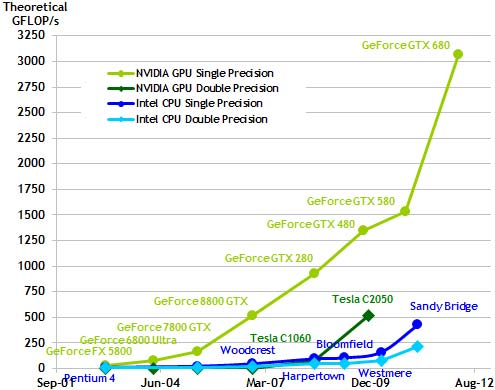
\includegraphics[width=0.7\linewidth]{../images/gpu_vs_cpu}
	\caption[Evolución de las GPUs respecto a las CPUs]{Evolución hasta 2012 de las GPUs respecto a las CPUs}
	\label{fig:gpu_vs_cpu}
\end{figure}


\bigskip
El uso de computación paralela, junto la potencia y la posibilidad de usar el paralelismo que ofrecen las GPU  hace muy interesante el uso de dichas GPUs para resolver algoritmos genéticos de formas más eficiente.

Después del estudio realizado en el siguiente capítulo, se opta por usar la arquitectura de cálculo CUDA \cite{nvidiacuda} para crear algoritmos genéticos que se ejecuten en GPUs de NVIDIA \cite{nvidiadeveloper}.

Como se cita en uno de los objetivos, se publicará de manera que cualquier usuario tenga acceso. Esto, junto a una interfaz sencilla, permitirá computar algoritmos genéticos con facilidad y rapidez.





\chapter{Estado del arte}
\bigskip

Los principios básicos de los algoritmos genéticos fueron establecidos por Holland (1975), y se encuentran bien descritos en varios textos a lo largo de los años, como los estudios de Goldberg (1989), Davis (1991), Michalewicz (1992) o Reeves (1993), afianzando los conceptos y permitiendo trabajar sobre una buena base a futuros investigadores.

\bigskip
Son muchos y muy variados los ámbitos en los que se usan los algoritmos genéticos. Sirven para crear componentes automovilísticos, analizar expresiones de genes o hasta desarrollar aprendizajes de comportamiento para robots, por ejemplo. Incluso se usan en aquellos que otros métodos no consiguen resolver o tiene problemas, o dichos métodos se pueden llegar a conjuntar con los algoritmos genéticos para así mejorarlos.

\bigskip
Aunque no se garantiza que el algoritmo genético encuentre la solución óptima del problema, éste encontrará soluciones de un nivel aceptable, en un tiempo competitivo con el resto de los algoritmos de optimización combinatoria. 

\bigskip
Esto hace que se estudie y se intente mejorar y optimizar dichos algoritmos, siendo un campo con mucha transcendencia en la actualidad.

\bigskip
Constan de varias partes, como la selección de candidatos, operadores de cruce, funciones de evaluación y optimización o mutación. En este trabajo nos centraremos en la parte de optimización, donde se evalúan los individuos generados y que serán posibles soluciones al problema. Existen multitud de funciones de optimización, pero nos centraremos en 2: Ackley y Rastrigin.

\bigskip
La función de Ackley se publicó por primera vez en ``A connectionist machine for genetic hillclimbing`` por David H. Ackley en 1987 y se extendió a la dimensión arbitraria en ``Evolutionary algorithms in theory and practice: evolution strategies, evolutionary programming, genetic algorithms`` por Thomas Bäck en 1996.

\bigskip
\begin{figure}[h]
	\centering
	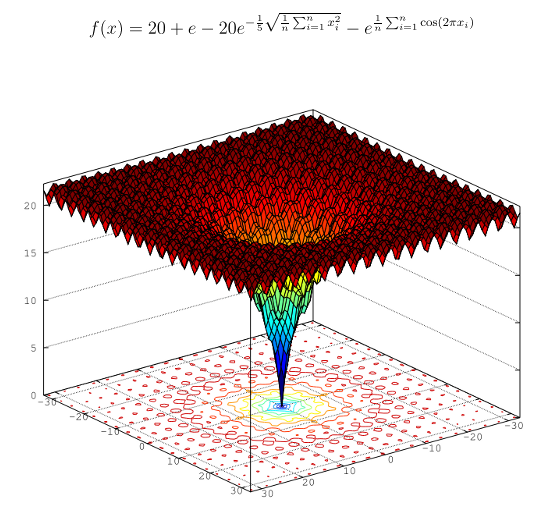
\includegraphics[width=0.7\linewidth]{../images/ackley}
	\caption[Función y representación de la función de optimización de Ackley]{Función y representación de la función de optimización de Ackley}
	\label{fig:ackley}
\end{figure}


\bigskip
Años antes, en 1974, Rastringin en "Systems of extremal control" propone otra función de optimización, para ser generalizada en 1991 por Mühlenbein.

\bigskip
\begin{figure}[h]
	\centering
	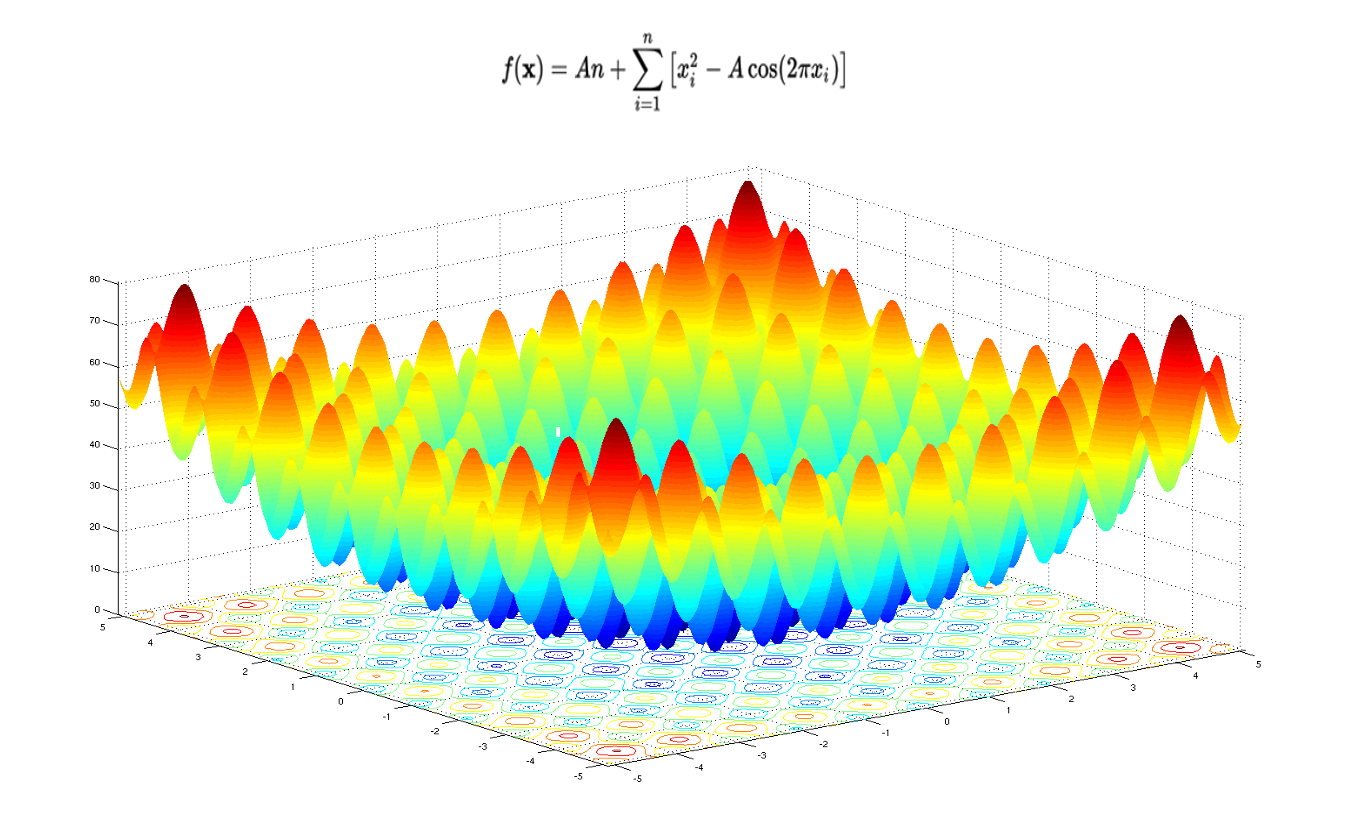
\includegraphics[width=0.7\linewidth]{../images/rastrigin}
	\caption[Función y representación de la función de optimización de Rastrigin]{Función y representación de la función de optimización de Rastrigin}
	\label{fig:rastrigin}
\end{figure}

\bigskip
Este trabajo se centrará en estas 2 funciones de optimización, ofreciendo un algoritmo genético que pueda ser optimizado mediante Ackley o Rastrigin.



\newpage
\section{Actualidad}
\bigskip

En la actualidad la mayoría de los usuarios que necesitan procesar un algoritmo genético lo hacen ellos mismos, con programas adaptados de terceros o desarrollados por ellos mismos. Esto conlleva un trabajo extra de estudio, implementación y corrección de dichos programas. 

Podemos encontrar algunos programas \cite{agpython} \cite{agjava} \cite{agmatlab} para ser ejecutados por el cliente, o servicios web que realizan algoritmos genéticos donde la mayoría son ejemplos o demostraciones de algoritmos genéticos y sus soluciones \cite{agandar} \cite{agcoche}.


Pero ninguno usa la computación paralela aprovechando la potencia de las GPUs. Viendo que hay disponible en el ámbito de dicha paralelización vemos que hay grandes empresas que han lanzado lenguajes de programación enfocados a aprovechar el procesamiento mediante la GPU: CUDA \cite{nvidiacuda}, AMD OpenCL APP \cite{paralelizacionamd}, BrookGPU \cite{brookgpu}, PeakStream \cite{peackstream} o RapidMind \cite{rapidmind}:

\begin{itemize}
	\item CUDA: arquitectura de cálculo paralelo de NVIDIA. Se basa en el lenguaje C y C++, por lo que, junto con la cantidad de dispositivos de la marca, existe una gran comunidad y documentación.
	
	\item AMD OpenCL™ Accelerated Parallel Processing: herramienta de AMD que permite el cómputo mediante GPUs. Se basa en los lenguajes OpenCL y C++, por lo que se pueden usar para acelarar aplicaciones.
	
	\item BrookGPU: programa (en versión \textit{beta}) de la Universidad de Stanford para aprovechar la paralelización en tarjetas gráficas AMD y NVIDIA. Para trabajar con el se usa una extensión de ANSI C.
	
	\item PeakStream era un programa para paralelizar el procesamiento con grandes rendimientos en tarjetas AMD, comprado por Google en 2007 \cite{peackstreamcomprada}, y tras esto, a dejado de ofrecer mantenimiento.
	
	\item RapidMind, que tambíen se basa en C++, es comprada por Intel en 2009 y pasa a ser Intel Array Building Blocks \cite{rapidmindcomprada}, pero sigue estando en forma experimental. 
	
\end{itemize}

Tras ver las distintas opciones, con sus distintas ventajas e inconvenientes, se decide centrar en CUDA. Es un proyecto activo, tiene numerosas actualizaciones, cuenta con mucha comunidad para resolver dudas y fomentar su desarrollo, y tiene numerosas facilidades, como un SDK \cite{nvidiadeveloper} y varias herramientas para sus desarrolladores. Por todo esto se escoge CUDA para desarrollar el trabajo.

\bigskip
CUDA surgió en 2006, cuando NVIDIA lanzó por primera vez al mercado una GPU capaz de renderizar gráficos en 3D y que incluyó la posibilidad de ejecutar, usando CUDA, programas escritos en lenguaje C.

\bigskip
\begin{figure}[h]
	\centering
	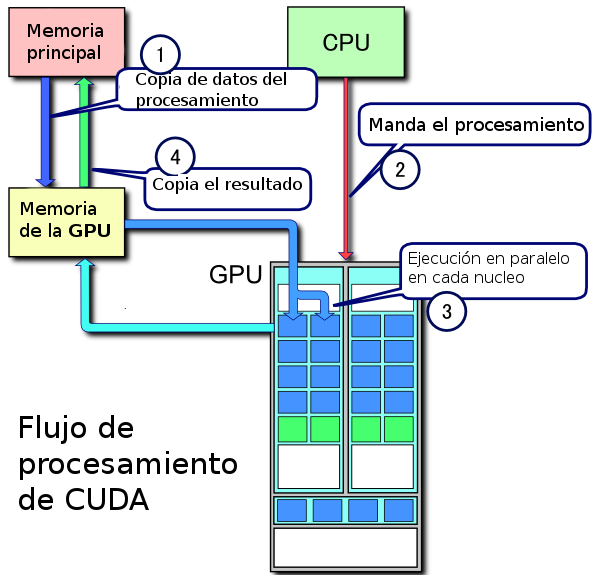
\includegraphics[width=0.6\linewidth]{../images/flujocuda}
	\caption[Ejemplo de flujo de procesamiento  CUDA]{Ejemplo de flujo de procesamiento CUDA}
	\label{fig:flujocuda}
\end{figure}


Gracias a su eficiencia energética y gran potencia, desde entonces NVIDIA ofrece la capacidad de sus tarjetas gráficas para grandes centros de datos y otras instituciones tanto científicas como gubernamentales, permitiendo dibujar gráficos y ejecutar diversos programas aprovechando.

Incluso se utilizan versiones reducidas para potenciar las aplicaciones tanto de teléfonos móviles, ordenadores portátiles y tablets, entre
otros.


\bigskip
En este campo hay algunos proveedores, como Impact  \cite{cudaimpact} o gpuOcelot \cite{cudagpuocelot} que ofrecen herramientas para la computación de algoritmos estándar o del código que genere el usuario, pero  realizando el cómputo desde las GPUs de los clientes, y nunca enfocados específicamente a resolver algoritmos genéticos.

\bigskip
Otras opciones permiten ejecutar CUDA en servidores externos, pero se necesita enviar una solicitud de uso y adaptarse a sus restricciones y capacidad, como en rCUDA \cite{rcuda}
o desplegar toda una instancia en un IaaS y desarrollar dentro: Amazon Web Services \cite{amazoncuda}.

\bigskip
Con esto se puede ver que podemos encontrar servicios que realicen algoritmos genéticos, o servicios que usen CUDA, pero no hay servicios que combinen ambos.


\bigskip
\section{Clientes}
\bigskip

¿Que usuarios necesitan computar algoritmos genéticos?

Por ejemplo, cualquier estudiante que quiera comprobar los distintos resultados del algoritmo genético cambiando sus parámetros. También el personal de investigación trabaja con multitud de algoritmo genéticos, y con grandes consumos de recursos. Junto con la potencia de cómputo y la accesibilidad que proporcionaremos simplificaríamos el trabajo de dicho personal. 

Además el servicio será accesible a cualquier usuario, y con su interfaz sencilla e intuitiva dichos usuarios no necesitarán una preparación especial para usarlo. 

\bigskip
\section{Competidores}
\bigskip

Como se cita antes, existen ejemplos o plantillas de algoritmos genéticos \cite{agpython} \cite{agjava} \cite{agmatlab} que los usuarios pueden usar, pero necesitan para su uso un trabajo extra para su instalación, desarrollo o ajustes. Además de este trabajo extra, se ven limitados por las capacidades de sus dispositivos, pues los algoritmos se tendrán que lanzar en local.

Para evitar dichas limitaciones, podemos usar la paralelización de los algoritmos, pero los trabajos que encontramos se encuentran en una versión de CUDA obsoleta \cite{paralelizacioncuda} (y simplemente exponiendo el código) o son estudios del servicio sin llegar a ser implementado \cite{optimizacionparalelizacioncuda}. Se busca entonces un servicio que ofrezca computación desde un servidor externo. Se pueden ver servicios que computan directamente CUDA \cite{rcuda} u ofrecen instancias con acceso a GPUs \cite{amazoncuda}  pero nunca especializados en algoritmos genéticos.


\bigskip
\section{Conclusiones}
\bigskip

Si se busca un servicio de computación externo (que ofrezca una mayor potencia de computación usando GPUs) de algoritmos genéticos no llegamos a encontrar nada que cumpla con nuestro requisitos: o son servicios en local para lanzar algoritmos genéticos o son servicios externos que nos ofrecen computación aprovechando la paralelización de CUDA, pero sin llegar a ofrecer ninguna aproximación de un algoritmo genético.

Viendo esto se encuentra una demanda que podemos cubrir con nuestro servicio, motivando a su análisis y desarrollo.








\chapter{Resolución del trabajo}

\bigskip
La planificación del proyecto se realizó al inicio del mismo y luego se fue alterando según las desviaciones que se producían. El inicio del proyecto fue el 1 de Abril, aunque hasta el 1 de Julio se trabajó en él de manera entrecortada y sin profundidad, y la fecha de fin planificada es el 10 de Septiembre. 

Se podrán distinguir varias etapas en el trabajo, que se ven mejor en la siguiente imagen (Figura \ref{fig:gantt_previsto}) de la planificación:

\begin{itemize}
	\item Preparación y análisis: Aquí se hizo un análisis inicial del proyecto, con tecnologías a usar y un estudio más profundo de algunos conceptos vistos en el curso que se abordarían.
	
	\item Desarrollo del algoritmo genético: esta etapa consta de varias partes, ya que primero se trabajó con distintos algoritmos simples, genéticos o que usaban la paralelización a forma de formación y para facilitar un posterior diseño y análisis del algoritmo que se implementará. A medida que se acababa la implementación del algoritmo final, se hicieron pruebas con los resultados de ambas funciones de optimización.
	
	\item Desarrollo del servicio web: también consta de varias etapas. Primero se creo el BackEnd, y como el FrontEnd requería de los resultados del algoritmo, no se desarrolló hasta obtener algún resultado de este. Una vez completadas estas partes, se pasa al despliegue con una versión estable.
	
	\item Documentación: Aunque se ha ido preparando y almacenando información y recursos durante todo el trascurso del trabajo, la mayor parte de la memoria del trabajo se crea y se plasma en este documento en la etapa final, haciendo las correcciones y mejoras pertinentes.
\end{itemize}
 




\newpage
\section{Planificación}

A continuación se muestra mediante un diagrama de Gantt la planificación estimada del trabajo.

\bigskip
\begin{figure}[h]
	\centering
	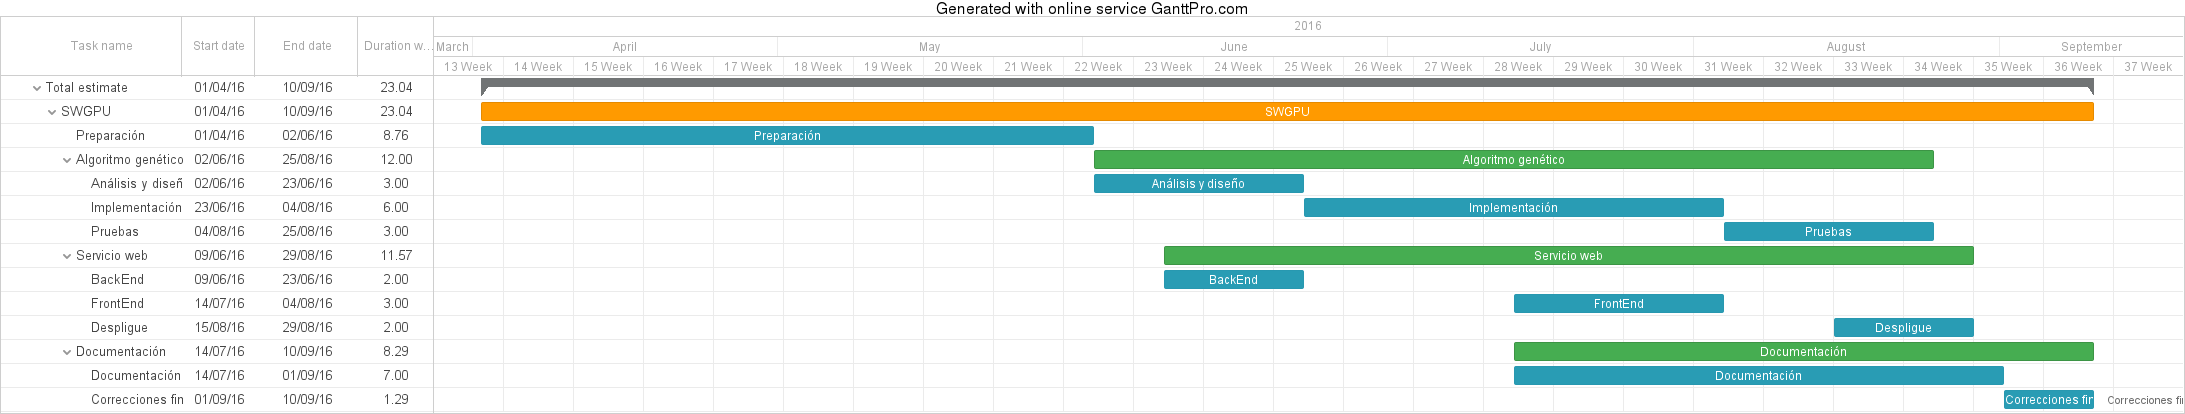
\includegraphics[width=1.0\linewidth]{../images/gantt_prevista}
	\caption[Diagrama Gantt de la planificación prevista del trabajo]{Diagrama Gantt de la planificación prevista del trabajo}
	\label{fig:gantt_previsto}
\end{figure}

\bigskip
Y en la siguiente figura se ve el desarrollo que se a producido, tras desviaciones imprevistas o ajustes de tiempo durante el mismo proceso:


(aproximación del diagrama de Gantt, pendiente la definitiva:)


\bigskip
\begin{figure}[h]
	\centering
	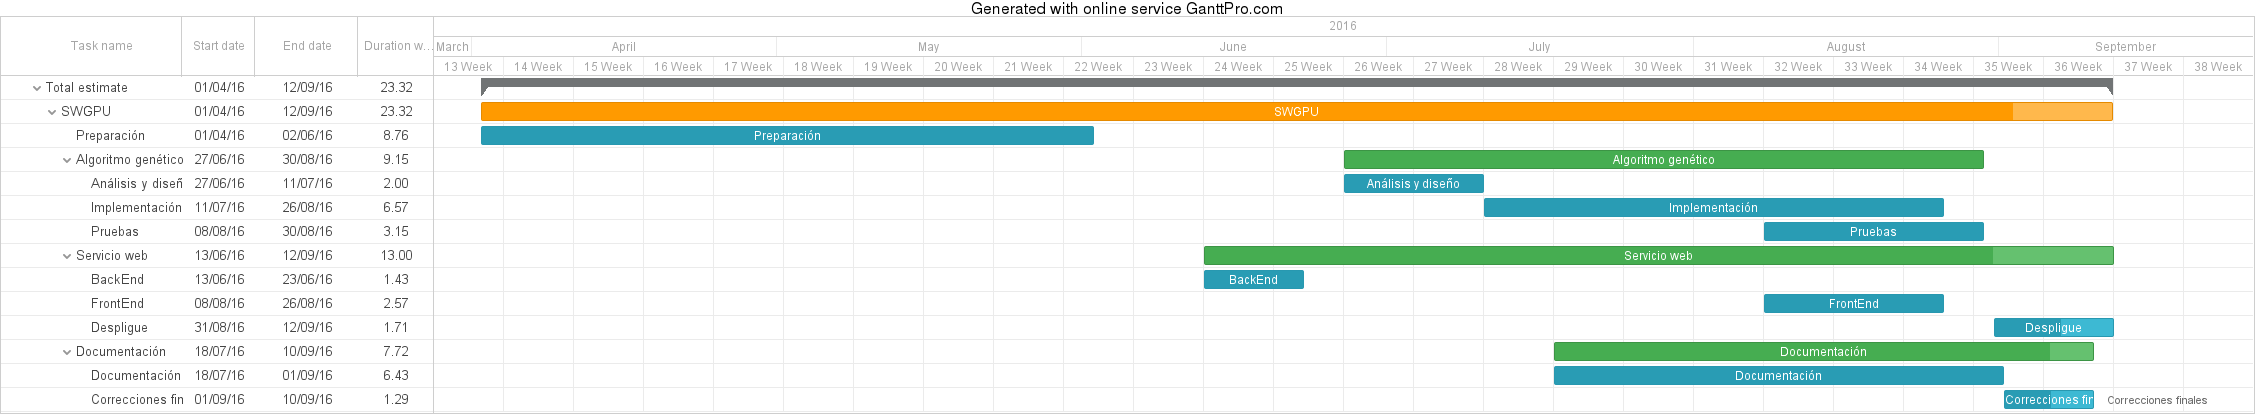
\includegraphics[width=1.0\linewidth]{../images/gantt}
	\caption[Diagrama Gantt de la planificación del trabajo]{Diagrama Gantt de la planificación del trabajo}
	\label{fig:gantt}
\end{figure}


\bigskip
\subsection{Conteo de horas y presupuesto}
\bigskip

\textbf{Conteo de horas}

\begin{itemize}
	
	\item Estimado
		\begin{itemize}
			\item Preparación: 
	
			8.75 semanas, a 3 días/semana, a 2 horas/día: 52.5 horas	
			
			\item Desarrollo de algoritmo genético: 
			
			12 semanas, a 4 días/semana, a 4 horas/día:  192 horas

			\item Desarrollo de servicio web: 
			
			7 semana, a 5 días/semana, a 2 horas/día: 70 horas
			
			\item Documentación: 
			
			8.29 semanas, a 4 días/semana, a 2 horas/día: 66.3 horas
			
			\bigskip			
			\textbf{Con lo que se sumaría un total de 380.8 horas.}
			
		\end{itemize}
	
	\item Real
		\begin{itemize}
			\item Preparación: 
			
			8.76 semanas, a  3 días/semana, a  2 horas/día:  52.5 horas
			
			\item Desarrollo de algoritmo genético: 
			
			9.15 semanas, a 4 días/semana, a 4 horas/día: 146.4 horas
			
			\item Desarrollo de servicio web: 
			
			?? semanas, a 5 días/semana, a 2 horas/día:  ?? horas
			
			\item Documentación: 
			
			?? semanas, a 4 días/semana, a 2 horas/día: ?? horas
			
			\bigskip			
			\textbf{Sumando finalmente un total de ?? horas.}

		\end{itemize}
		
\end{itemize}

\bigskip
\textbf{Presupuesto}

En este punto veremos los presupuesto según el conteo de horas para cada una de las 2 estimaciones y los servicios que requiramos. Suponiendo la media actual de un programador Junior \cite{sueldos}: 9\officialeuro/hora


\bigskip
\begin{itemize}
	
	\item Estimado
	\begin{itemize}
		\item Preparación: 
		
		52.5 horas x 9\officialeuro/hora : 472,5\officialeuro
		
		\item Desarrollo de algoritmo genético: 
		
		192 horas x 9\officialeuro/hora: 1728\officialeuro
		
		\item Desarrollo de servicio web
		
		70 horas x 9\officialeuro/hora: 630\officialeuro
		
		\item Documentación: 

		66.3 horas x 9\officialeuro/hora: 596,7\officialeuro
		
		\item \textit{Instancia que permita usar CUDA}
		
		Se contratarán servicios externos de cómputo mediante CUDA \cite{amazoncuda} con un coste de 1.88\officialeuro/h (2.10\textdollar/h). Suponiendo que este servicio estuviese en total disponibilidad (24 horas los 7 días de la semana) alcanzaría en sólo un mes de servicio los 315,84\officialeuro.
		
		\item \textit{Dominio para alojar una web publica del servicio}
		
		En caso de que no fuese posible, se contrataría un dominio por precios de 2.08\officialeuro a 4.95\officialeuro al mes (con permanencia de 12 meses, en las webs de alojamiento \textit{Hostpapa.es} \cite{hostpapa} y \textit{Dondominio.com} \cite{dondominio})
		
		\bigskip
		\textbf{Presupuesto total estimado: 3745,12\officialeuro (para el desarrollo y sólo un mes en producción) }
		
	\end{itemize}
	
	\item Real
	\begin{itemize}
		\item Preparación
		
		52.5 horas 9\officialeuro/hora
		
		\item Desarrollo de algoritmo genético
		
		146.4 horas 9\officialeuro/hora
		
		\item Desarrollo de servicio web
		
		?? x 9\officialeuro/hora
		
		\item Documentación

		?? x 9\officialeuro/hora
		
		\item \textit{Instancia que permita usar CUDA}
		
		En esta parte se aprovechará el servidor que ofrece la tutora del trabajo {\tutor}, con gran capacidad de cómputo y de manera gratuita. Esto ayudará de manera muy importante al trabajo, ya que reducirá de manera muy importante el presupuesto final del proyecto.
		
		\item \textit{Dominio para alojar una web publica del servicio}
		
		Al igual que en el punto anterior, se aprovechará el servicio de la tutora para lanzar el servicio web, reduciendo también el presupuesto final.
		
		\bigskip
		\textbf{Presupuesto total real: ? \officialeuro}
		
	\end{itemize}

\end{itemize}



\newpage
\section{Tecnologías}

En este apartado se describirán las tecnologías utilizadas en el trabajo. Se desglosarán después de listarlas:

\bigskip
En la parte del servidor:
\begin{itemize}
	\item Python
	\item Django
	\item Apache
	\item C++
	\item CUDA
\end{itemize}

Y de cara al cliente:
\begin{itemize}
	\item HTML5
	\item CSS3
	\item JavaScript
	\item AngularJS
	\item jQuery
	\item JSON
	\item HTML5UP
\end{itemize}

\bigskip
\subsection{Servidor}
\bigskip

\begin{itemize}
	\item \textbf{Python}
	
		Versión usada: 2.7.6
		
		Python \cite{python} es un lenguaje de programación interpretado cuya filosofía hace hincapié en una sintaxis que favorezca un código legible, además de simple y versátil.
				
		\bigskip
		\begin{figure}[h]
			\centering
			
\includegraphics[width=0.2\linewidth]{../images/python}
			\caption[Logo de Python]{Logo de Python}
			\label{fig:pythonlogo}
		\end{figure}
		
		Se trata de un lenguaje de programación multiparadigma, ya que soporta orientación a objetos, programación imperativa y, en menor medida, programación funcional. Es un lenguaje interpretado, usa tipado dinámico y es multiplataforma.
		
	\item \textbf{Django}
	
		Versión usada: 1.10
		
		Django \cite{django} es un framework de alto nivel web de Python. Fomenta el rápido desarrollo y un diseño limpio y pragmático. Se encarga de facilitar la creación de aplicaciones web complejas, ofreciendo las funcionalidades básicas y más útiles al desarrollador, para que pueda centrarse en la escritura de su aplicación.
		
		\bigskip
		\begin{figure}[h]
			\centering
			
\includegraphics[width=0.3\linewidth]{../images/djangologo}
			\caption[Logo de Django]{Logo de Django}
			\label{fig:djangologo}
		\end{figure}
				
	\item Apache
	
		Versión usada: 2.4.12
		
		El servidor HTTP Apache \cite{apache} es un servidor web de código abierto, multiplataforma, extensible y modular. Además, al ser tan popular tiene un gran soporte de la comunidad.
		
		Implementa el protocolo HTTP y la noción de sitio virtual. 
		

		\bigskip
		\begin{figure}[h]
			\centering
			
\includegraphics[width=0.4\linewidth]{../images/apachelogo}
			\caption[Logo de Apache]{Logo de Apache}
			\label{fig:apachelogo}
		\end{figure}
				
	\item \textbf{C++}
	
	Versión usada: 4.8.8
	
	C++ \cite{cpp} es un lenguaje de programación que extiende a C añadiendo mecanismos que permiten la manipulación de objetos. 
	
	Tiene las facilidades de programación genérica junto a los paradigmas de programación estructurada y programación orientada a objetos. 
		 
	
	\item \textbf{CUDA}
	
	Versión usada: 7.5
	
	CUDA \cite{nvidiacuda} es una arquitectura de cálculo paralelo de NVIDIA que aprovecha la gran potencia de la GPU (unidad de procesamiento gráfico) para proporcionar un incremento extraordinario del rendimiento del sistema.
	
	Dispone de una gran comunidad, ya que es la arquitectura de cálculo paralelo más usada en la actualidad, en parte gracias a su potencia y la facilidad de uso para los desarrolladores.

	
	La plataforma de cálculo paralelo CUDA proporciona unas cuantas extensiones de C y C++ que permiten implementar el paralelismo en el procesamiento de tareas y datos con diferentes niveles de granularidad y con la flexibilidad de usar varios lenguajes, como son C, C++ y Fortran. 
	
	Dispone de numerosas facilidades para los desarrolladores, como herramientas de desarrollo, documentación y su \textit{toolkit}.

		\bigskip
		\begin{figure}[h]
			\centering
			
\includegraphics[width=0.3\linewidth]{../images/cudalogo}
			\caption[Logo de CUDA]{Logo de CUDA}
			\label{fig:cudalogo}
		\end{figure}
	
			
\end{itemize}
	

\newpage
\subsection{Cliente}
\bigskip


\begin{itemize}
	\item \textbf{HTML5}
	
	HTML (HyperText Markup Language) \cite{html} en su la quinta revisión, es el lenguaje básico de la World Wide Web. Es un estándar que sirve de referencia de elaboración de páginas web en sus diferente versiones. Define una estructura básica y un código para la definición de contenido de una página web, como texto, imágenes o vídeos. Usa un sistema para formatear el layout de nuestras páginas, así como hacer algunos ajustes a su aspecto. Los navegadores como Chrome, Firefox, Explorer o Safari puede saber como representar el contenido de una web, con las ubicaciones de todos los elementos.
	
	
	\bigskip
	\begin{figure}[h]
		\centering
		
\includegraphics[width=0.3\linewidth]{../images/htmllogo}
		\caption[Logo de HTML5]{Logo de HTML5}
		\label{fig:htmllogo}
	\end{figure}
	
	\item \textbf{CSS3}
		
	 CSS (Cascading Style Sheets) \cite{css} u hoja de estilo en cascada, es un lenguaje usado para definir y crear la presentación de un documento estructurado escrito en HTML o XML2. El World Wide Web Consortium (W3C) es el encargado de formular la especificación de las hojas de estilo, al igual que del lenguaje HTML, que servirán de estándar para los agentes de usuario o navegadores.

	 Aunque la información de estilo puede ser definida en el mismo documento HTML, la idea que se encuentra detrás del desarrollo de CSS es separar la estructura de un documento de su presentación. 

	
	\bigskip
	\begin{figure}[h]
		\centering
		
\includegraphics[width=0.3\linewidth]{../images/csslogo}
		\caption[Logo de CSS3]{Logo de CSS3}
		\label{fig:csslogo}
	\end{figure}
		
	\item \textbf{JavaScript}
		
	JavaScript \cite{js} es un lenguaje de programación interpretado, que se define como orientado a objetos, basado en prototipos, imperativo, débilmente tipado y dinámico.

	Se utiliza principalmente en su forma del lado del cliente, implementado como parte de un navegador web permitiendo mejoras en la interfaz de usuario y páginas web dinámicas (aunque existe una forma de JavaScript del lado del servidor). 

	Todos los navegadores modernos interpretan el código JavaScript integrado en las páginas web. Para interactuar con una página web se provee al lenguaje JavaScript de una implementación del Document Object Model (DOM).

	\bigskip
	\begin{figure}[h]
		\centering
		
\includegraphics[width=0.3\linewidth]{../images/jslogo}
		\caption[Logo de JavasSript]{Logo de JavaScript}
		\label{fig:jslogo}
	\end{figure}
			
	\item \textbf{AngularJS}
		
	Versión usada: 1.5.7
		
	AngularJS \cite{angularjs} es un framework de JavaScript de código abierto, mantenido por Google, que se utiliza para crear y mantener aplicaciones web de una sola página. Su objetivo es aumentar las aplicaciones basadas en navegador con capacidad de Modelo Vista Whatever (MVW), en un esfuerzo para hacer que el desarrollo y las pruebas sean más fáciles.

	La biblioteca lee el HTML que contiene atributos de las etiquetas personalizadas adicionales, entonces obedece a las directivas de los atributos personalizados, y une las piezas de entrada o salida de la página a un modelo representado por las variables estándar de JavaScript, que además se pueden configurar manualmente, o recuperados de los recursos JSON estáticos o dinámico

	\bigskip
	\begin{figure}[h]
		\centering
		
\includegraphics[width=0.4\linewidth]{../images/angularjslogo}
		\caption[Logo de AngularJS]{Logo de AngularJS}
		\label{fig:angularjslogo}
	\end{figure}
		
	\item \textbf{jQuery}
	
		Versión usada: 1.11.3
		
	jQuery \cite{jquery} es una biblioteca de JavaScript que permite simplificar la manera de interactuar con los documentos HTML, manipular el árbol DOM, manejar eventos, desarrollar animaciones y agregar interacción con la técnica AJAX a páginas web.

	jQuery, al igual que otras bibliotecas, ofrece una serie de funcionalidades basadas en JavaScript de manera muy reducida, por lo que con las funciones propias de esta biblioteca se logran grandes resultados en menos tiempo y espacio. Todo esto hace que sea la biblioteca JavaScript más usada.
		
	\bigskip
	\begin{figure}[h]
		\centering
		
\includegraphics[width=0.4\linewidth]{../images/jquerylogo}
		\caption[Logo de jQuery]{Logo de jAuery}
		\label{fig:jquerylogo}
	\end{figure}
		
	\item \textbf{JSON}
		
	JSON (JavaScript Object Notation) \cite{json} es un formato ligero de intercambio de datos. Gracias a su sencillez es fácil leerlo y escribirlo para humanos, mientras que para las máquinas es simple interpretarlo y generarlo.
	
	Es un formato de texto que es completamente independiente del lenguaje pero utiliza convenciones que son ampliamente conocidos por los programadores de los principales lenguajes. 
	
	Estas propiedades hacen que JSON sea un lenguaje ideal para el intercambio de datos.

	\bigskip
	\begin{figure}[h]
		\centering
		
\includegraphics[width=0.3\linewidth]{../images/jsonlogo}
		\caption[Logo de JSON]{Logo de JSON}
		\label{fig:jsonlogo}
	\end{figure}
	
	\item \textbf{HTML5UP}
		
	HTML5UP \cite{htmlup} Web con múltiples plantillas disponibles (usando HTML y JavaScript) y estilos CSS con los que crear la estructura básica de proyectos web. Son completamente personalizables y	tienen un diseño web adaptable (\textit{responsive}) de manera que la web que creemos se adaptará a cualquier pantalla, punto muy importante en la actualidad, debido a la multitud de dispositivos y tamaños de pantalla que existen.

	\bigskip
	\begin{figure}[h]
		\centering
		
\includegraphics[width=0.3\linewidth]{../images/htmluplogo}
		\caption[Logo de HTML5UP]{Logo de HTML5UP}
		\label{fig:htmluplogo}
	\end{figure}
		
\end{itemize}
	
	
	

\newpage
\section{Herramientas}

En este apartado se listarán y desglosarán las herramientas usadas para usar las tecnologías anteriores.


\begin{itemize}
	\item \textbf{Nsight Eclipse Edition}
	
	Versión usada: 7.5
		
	Nsigh (NVIDIA Nsight Eclipse Edition) \cite{nsight} es la gran plataforma de desarrollo para cálculo heterogéneo. Permite trabajar con potentes herramientas de depuración y análisis del rendimiento para optimizar el funcionamiento de la CPU y la GPU. Esta plataforma permite optimizar el rendimiento de manera intuitiva, identificar y analizar los cuellos de botella y observar el comportamiento de todas las actividades del sistema.

	Consta de varias plantillas y ejemplos, además de estar disponible varios sistemas operativos.
 
	\bigskip
	\begin{figure}[h]
		\centering
		
\includegraphics[width=0.5\linewidth]{../images/nsightlogo}
		\caption[Logo de Nsight]{Logo de Nsight}
		\label{fig:nsightlogo}
	\end{figure}
	
	\item \textbf{TeXstudio}
		
		Versión usada: 2.11.0
		
	TeXstudio \cite{texstudio} es un entorno de escritura para la creación de documentos LaTeX de manera fácil, cómoda e intuitiva. Tiene numerosas características, como el resaltado de sintaxis, pre-visualizador integrado, verificación de referencias y varios asistentes. 

	Tiene una gran documentación y comunidad, además de estar disponible para los sistemas operativos más importantes.
		
	\bigskip
	\begin{figure}[h]
		\centering
		
\includegraphics[width=0.3\linewidth]{../images/texstudiologo}
		\caption[Logo de TeXstudio]{Logo de TeXstudio}
		\label{fig:texstudiologo}
	\end{figure}
			
	\item \textbf{Git}
			
		Versión usada: 1.91
		
	Git \cite{git} es un software de control de versiones, pensando en la eficiencia y la confiabilidad del mantenimiento de versiones de aplicaciones cuando éstas tienen un gran número de archivos de código fuente. 

	Git se considera un sistema de control de versiones con funcionalidad plena y con multitud de características, como la gestión distribuida o la rápida gestión de ramas. 

	\bigskip
	\begin{figure}[h]
		\centering
		
\includegraphics[width=0.3\linewidth]{../images/gitlogo}
		\caption[Logo de Git]{Logo de Git}
		\label{fig:gitlogo}
	\end{figure}
				
	\item \textbf{Sublime Text}
			
	Versión usada: 2, versión de evaluación
		
	Sublime Text \cite{sublimetext} es un editor de texto y de código fuente. Originalmente fue desarrollado como una extensión de Vim y con el tiempo fue creando una identidad propia.

	Poseee varias características para los desarrolladores, como un \textit{minimapa} del código, multi-selección y multi-cursor, búsqueda dinámica y soporte a multitud de lenguajes.


	\bigskip
	\begin{figure}[h]
		\centering
		
\includegraphics[width=0.3\linewidth]{../images/sublimetextlogo}
		\caption[Logo de Sublime Text]{Logo de Sublime Text}
		\label{fig:sublimetextlogo}
	\end{figure}
				
	\item \textbf{Gimp}
			
	Versión usada: 2.8.10
		
	GIMP (GNU Image Manipulation Program) \cite{gimp} es un programa de edición de imágenes digitales en forma de mapa de bits, tanto dibujos como fotografías. 

	Tiene multitud de herramientas para el retoque y edición de imágenes o un dibujo libre.

	Esta disponible para la mayoría de los sistemas operativos y en varios lenguajes.

	\bigskip
	\begin{figure}[h]
		\centering
		
\includegraphics[width=0.3\linewidth]{../images/gimplogo}
		\caption[Logo de Gimp]{Logo de Gimp}
		\label{fig:gimplogo}
	\end{figure}
	
	
	\item \textbf{GanttPRO}
	
	GanttPRO \cite{ganttpro} permite la gestión de proyectos mediante diagramas de Gantt.

	Mediante su interfaz se pude planificar y gestionar proyectos con facilidad con diagramas de Gantt, mediante tareas, subtareas o duraciones dinámicas. 	

	\bigskip
	\begin{figure}[h]
		\centering
		
\includegraphics[width=0.3\linewidth]{../images/ganttprologo}
		\caption[Logo de GanttPRO]{Logo de GanttPRO}
		\label{fig:ganttprologo}
	\end{figure}

	\item \textbf{Draw.io}
	
	Draw.io \cite{drawioweb} es una herramienta para crear varios tipos de diagramas, entre ellos del tipo UML.
	
	\bigskip
	\begin{figure}[h]
		\centering
		
\includegraphics[width=0.3\linewidth]{../images/drawiologo}
		\caption[Logo de Draw.io]{Logo de Draw.io}
		\label{fig:drawiologo}
	\end{figure}
					
\end{itemize}


\chapter{Descripción del sistema}

\bigskip
En este capítulo se describe la fase de análisis del proyecto. Algunos requisitos o partes del capítulo fueron modificados o corregidos durante el trabajo. A continuación se muestran los definitivos.

\bigskip
\section{Análisis inicial}

Este proyecto fue propuesto desde un principio por {\tutor}, ya que en su ámbito de investigación requiere algoritmos evolutivos con muchos requerimientos de cómputo, por lo que al  pararelizarlos se logran unos resultados más rápidos, y al estar disponible en un servicio web no es necesario un dispositivo específico.

Después de la propuesta del trabajo, y antes del desarrollo del mismo se hicieron diversas reuniones para establecer sus bases y alcance. 

En la selección de tecnologías a usar se optó por la arquitectura de cómputo CUDA, ya que es actualmente la más potente, como se ve en el capítulo anterior, y se dispone de una tarjeta gráfica NVIDIA de gran potencia.

En la parte del servicio web se optó por el framework python Django, ya que se estudió con profundidad a lo largo del curso y es en la actualidad es la mejor opción para realizar un servicio web.

Dichas tecnologías son actuales, con una gran comunidad detrás, de manera que están en continuo desarrollo y mejora, además de estar bien asentadas, dando robustez al trabajo.


\newpage
\section{Objetivos}

Este trabajo tiene como principal objetivo el desarrollo de unas clases que lancen algoritmos genéticos de forma paralela, y puedan ser usados por un servicio web.

Los principales objetivos, de manera reducida, que se quieren alcanzar con este trabajo son:


\begin{itemize}
	\item  \textbf{OBJ. 1} Gestión del servicio web
	\begin{itemize}
		\item \textbf{OBJ. 1.1} Ejecución de algoritmo genético.	
		\item \textbf{OBJ. 1.2} Consulta de la solución.
		\item \textbf{OBJ. 1.3} Contacto con el administrador o personal de contacto.
	\end{itemize}
		
	\item  \textbf{OBJ. 2} Gestión del algoritmo genético
	\begin{itemize}
		\item \textbf{OBJ. 2.1} Entrada de parámetros.
		\item \textbf{OBJ. 2.2} Ejecución del algoritmo genético.
		\item \textbf{OBJ. 2.3} Generar salida en formato JSON.
	\end{itemize}
	
\end{itemize}


	 

\newpage
\section{Especificación de requisitos}

\subsection{Requisitos funcionales}

\bigskip
En esta sección del capítulo se definirán las características de alto nivel (requisitos funcionales) del sistema que son necesarios para las necesidades del usuario.

\bigskip

\begin{itemize}
	\item  \textbf{RF. 1 Gestión del servicio web}
	\begin{itemize}
		\item \textbf{RF. 1.1} Ejecución de algoritmo genético.
		\begin{itemize}
			\item \textbf{RF. 1.1.1} Entrada de parámetros .
			\item \textbf{RF. 1.1.2} Petición al servidor.
		\end{itemize}
		
		\item \textbf{RF. 1.2} Consulta de la solución.
		\item \textbf{RF. 1.3} Contacto con el administrador o personal de contacto.
	\end{itemize}
	
	\item  \textbf{RF. 2 Gestión del algoritmo genético}
	\begin{itemize}
		\item \textbf{RF. 2.1} Entrada de parámetros.
		\item \textbf{RF. 2.2} Ejecución del algoritmo.
		\begin{itemize}
			\item \textbf{RF. 2.2.1} Generación de poblaciones.
			\item \textbf{RF. 2.2.2} Evaluación de cada individuo.
			\begin{itemize}
				\item \textbf{RF. 2.2.2.1} Evaluación mediante la función Ackley.
				\item \textbf{RF. 2.2.2.2} Evaluación mediante la función Rastrigin.
			\end{itemize}
			\item \textbf{RF. 2.2.3} Selección de individuos para el cruce.
			\item \textbf{RF. 2.2.4} Cruce de individuos.
			\item \textbf{RF. 2.2.5} Mutación del individuo.
			\item \textbf{RF. 2.2.6} Reemplazo del individuo.
		\end{itemize}
		\item \textbf{RF. 2.3} Generar salida en formato JSON.
	\end{itemize}
	
\end{itemize}



\bigskip
\subsection{Requisitos no funcionales}

\bigskip
En esta sección se establecen los requisitos no funcionales.

\bigskip
\textbf{Rendimiento}\\

\textbf{RNF 1}: Será implementado con tecnologías que optimicen el rendimiento y la eficacia, tanto en el servicio web como en el algoritmo genético.\\

\textbf{Disponibilidad}\\

\textbf{RNF 2}: Se intentará que el servicio esté disponible las 24 horas del día, con una estructura segura y preparada ante los fallos.\\


\textbf{Accesibilidad}\\

\textbf{RNF 3}: Se logrará una gran accesibilidad al tratarse de un servicio web.\\


\textbf{Usabilidad}\\

\textbf{RNF 4}: La interfaz, con el orden y disposición de los elementos será lo más usable posible.\\

\textbf{Interfaz}\\

\textbf{RNF 5}: La interfaz será sencilla e intuitiva.\\

\textbf{RNF 6}: Se adaptará a cualquier tamaño de pantalla, tendrá un diseño adaptativo.\\


\textbf{Estabilidad}\\

\textbf{RNF 7}: Se buscará la mayor estabilidad en el sistema, usando tecnologías robustas y estables.\\


\textbf{Mantenimiento}\\

\textbf{RNF 8}: Se ha desarrollado de manera ordenada y documentando todos las partes, para que el mantenimiento pueda ser realizado por el mismo desarrollador o por terceros de manera sencilla.\\


\textbf{Soporte}\\

\textbf{RNF 9}: Se le facilitará al usuario contacto con alguien responsable del sistema, para que en caso de necesitar soporto le sea fácil y rápido.\\


\bigskip
\subsection{Requisitos de información}

\bigskip
En esta sección se establecen los requisitos de información, que estarán fuertemente relacionados a los requisitos funcionales, ya que será la información mínima para llevarlos a cabo.

\begin{itemize}
	\item  \textbf{RI. 1 Gestión del servicio web}
	\begin{itemize}
		\item \textbf{RI. 1.1} Ejecución de algoritmo genético.
		\begin{itemize}
			\item Tamaño de la población
			\item Número de cromosomas
			\item Valor mínimo
			\item Valor máximo
			\item Probabilidad de cruce
			\item Probabilidad de mutación
			\item Número de generaciones
			\item Parámetros para la función Ackley
				\begin{itemize}
					\item Valor A
					\item Valor B
					\item Valor C 		
				\end{itemize}			
			\item Parámetros para la función Rastrigin
			\begin{itemize}
				\item Valor A
			\end{itemize}
		\end{itemize}
	\end{itemize}
		
	\item \textbf{RI. 1.2} Consulta de la solución.
	\begin{itemize}
		\item Hora de consulta
		\item Rendimiento
		\item Tiempo de cómputo
		\item Tamaño del cómputo
		\item Hebras usadas
		\item Datos de entrada (RI 1.1)
		\item Información del dispositivo que ha realizado el algoritmo
		\item Mejores variables obtenidas
		\item Mejor fitness
	\end{itemize}


	\item  \textbf{RI. 2 Gestión del algoritmo genético}
	\begin{itemize}
		\item \textbf{RI. 2.1} Entrada de parámetros.
		\begin{itemize}
			\item Dispositivo a usar
			\item Función de optimización a usar
			\item Tamaño de la población
			\item Número de cromosomas
			\item Valor mínimo
			\item Valor máximo
			\item Probabilidad de cruce
			\item Probabilidad de mutación
			\item Número de generaciones
			\item Parámetros para la función Ackley
				\begin{itemize}
					\item Valor A
					\item Valor B
					\item Valor C
				\end{itemize}
				
			\item RI 2.1.2 Parámetros para la función Rastrigin
				\begin{itemize}
					\item Valor A
				\end{itemize}
			\end{itemize}
		\end{itemize}

		\item \textbf{RI. 2.2} Generar salida en formato JSON.
		\begin{itemize}
			\item Rendimiento
			\item Tiempo de cómputo
			\item Tamaño del cómputo
			\item Hebras usadas
			\item Datos de entrada (RI 2.1)
			\item Información del dispositivo que ha realizado el algoritmo
			\item Mejores variables obtenidas
			\item Mejor fitness
		\end{itemize}
	
\end{itemize}


\bigskip
\subsection{Restricciones}

\bigskip
Las restricciones del sistema serán las siguientes:

\bigskip
\textbf{RSTR 1 Gestión del servicio web (Ejecución del algoritmo genético):}

\begin{itemize}
	\item RSTR 1.1: El tamaño de la población será menor de 10.000.
	\item RSTR 1.2: Habrá un máximo de 1.000 cromosomas (1.000 variables).
	\item RSTR 1.3: El valor máximo tendrá que ser más grande el el valor mínimo.
	\item RSTR 1.4: La probabilidad de cruce tendrá que ser entre 0 y 1.
	\item RSTR 1.5: La probabilidad de mutación tendrá que ser entre 0 y 1.
\end{itemize}


\bigskip
\textbf{RSTR 2 Gestión del algoritmo genético (Entrada de parámetros):}

\begin{itemize}
	\item RSTR 2.1: Para escoger la función con la que optimizar introducimos 0 o 1.
	\item RSTR 2.2: El tamaño de la población será menor de 10.000.
	\item RSTR 2.3: Habrá un máximo de 1.000 cromosomas (1000 variables).
	\item RSTR 2.4: El valor máximo tendrá que ser más grande el valor mínimo.
	\item RSTR 2.5: La probabilidad de cruce tendrá que ser entre 0 y 1.
	\item RSTR 2.6: La probabilidad de mutación tendrá que ser entre 0 y 1.
\end{itemize}


\newpage
\section{Modelo funcional}


\bigskip
\subsection{Resumen de actores}

\begin{itemize}
	\item \textbf{Usuario}
	
	Descripción: Representa al usuario que quiere hacer uso del sistema.\\
	
	Tipo: Primario\\
	
	Responsabilidad: Completar el formulario con los datos que requiera el algoritmo genético.
	
	\item \textbf{Administrador del sistema}
	
	Descripción: Representa a la persona encargada de mantener, actualizar y gestionar el sistema.\\
	
	Tipo: Secundario\\
	
	Responsabilidad: Realizar todas las actividades de gestión y actualización del sistema.
	
	\item \textbf{Servidor}
	
	Descripción: Representa al servidor, que realizará peticiones al sistema para ofrecérselas al Usuario.\\
	
	Tipo: Primario\\
	
	Responsabilidad: Ofrecer el servicio web al usuario y gestionar sus peticiones de cómputo.
	
\end{itemize}




\bigskip
\subsection{Identificación de los casos de uso}
\bigskip

Los distintos casos de uso serán:
\begin{itemize}
	\item Para la gestión del servicio web:
	\begin{itemize}

		\item \textbf{CU 1} Entrada de parámetros .
		\item \textbf{CU 2} Petición al servidor.	
		\item \textbf{CU 3} Consulta de la solución.
		\item \textbf{CU 4} Contacto con el administrador o personal de contacto.
	\end{itemize}
	
	\item Para la gestión del algoritmo genético:
	\begin{itemize}
		\item \textbf{CU 5} Entrada de parámetros.
		\item \textbf{CU 6} Generación de poblaciones.
		\item \textbf{CU 7} Evaluación mediante la función Ackley.
		\item \textbf{CU 8} Evaluación mediante la función Rastrigin.
		\item \textbf{CU 9} Selección de individuos para el cruce.
		\item \textbf{CU 10} Cruce de individuos.
		\item \textbf{CU 11} Mutación del individuo.
		\item \textbf{CU 12} Reemplazo del individuo.
		\item \textbf{CU 13} Generar salida en formato JSON.
	\end{itemize}
	
\end{itemize}



\bigskip
\subsection{Descripción de los casos de uso}
\bigskip


\begin{itemize}
	
	\item \textbf{CU 1} Entrada de parámetros.
	\begin{itemize}
		\item \textbf{Actores:} Usuario.
		\item \textbf{Tipo:} Primario, esencial.
		\item \textbf{Dependencias:}
		\item \textbf{Precondición:}
		\item \textbf{Postcondición:} El sistema hace una petición al servidor con los parámetros introducidos.
		\item\textbf{ Autor:} {\autor}.
		\item \textbf{Versión:} 1.0.
		\item \textbf{Propósito:} Especificar los parámetros del algoritmo genético.
		\item \textbf{Resumen:} El usuario introduce los parámetros (distintos a los declarados por defecto) que quiere para ejecutar el algoritmo genético. 
	\end{itemize}
	
	\item \textbf{CU Petición al servidor} .
	\begin{itemize}
		\item \textbf{Actores:} Usuario.
		\item \textbf{Tipo:} Primario, esencial.
		\item \textbf{Dependencias:} CU 1.
		\item \textbf{Precondición:} Los parámetros introducidos deben ser correctos.
		\item \textbf{Postcondición:} Se mandará una petición de cómputo al sistema que devolverá a la web.
		\item\textbf{ Autor:} {\autor}.
		\item \textbf{Versión:} 1.0.
		\item \textbf{Propósito:} Confirmar la petición al servidor.
		\item \textbf{Resumen:} El usuario realiza la petición de ejecución del algoritmo genético que busca.
	\end{itemize}

	\item \textbf{CU 3} Consulta de la solución.
	\begin{itemize}
		\item \textbf{Actores:} Usuario.
		\item \textbf{Tipo:} Primario, esencial.
		\item \textbf{Dependencias:} CU 2.
		\item \textbf{Precondición:} El usuario ha hecho la petición al servidor y este haber acabado.
		\item \textbf{Postcondición:} Resultados visibles al usuario
		\item\textbf{ Autor:} {\autor}.
		\item \textbf{Versión:} 1.0.
		\item \textbf{Propósito:} Permitir ver al usuario los resultados generados por el sistema.
		\item \textbf{Resumen:} Una vez que se resuelve el algoritmo genético, el servidor devuelve la solución, maquetada para facilitar su consulta al usuario.
	\end{itemize}

	\item \textbf{CU 4} Contacto con el administrador o personal de contacto.
	\begin{itemize}
		\item \textbf{Actores:} Usuario.
		\item \textbf{Tipo:} Opcional.
		\item \textbf{Dependencias:} 
		\item \textbf{Precondición:}
		\item \textbf{Postcondición:} El usuario podrá comunicarse con alguien encargado del sistema.
		\item\textbf{ Autor:} {\autor}.
		\item \textbf{Versión:} 1.0.
		\item \textbf{Propósito:} Poder notificar dudas o sugerencias del sistema.
		\item \textbf{Resumen:} El usuario podrá mandar un correo o ponerse en contacto con alguien responsable del sistema al usuario, pudiendo notificar así fallos o sugerencias sobre el sistema.
	\end{itemize}	

\bigskip

	\item \textbf{CU 5} Entrada de parámetros.
	\begin{itemize}
		\item \textbf{Actores:} Servidor.
		\item \textbf{Tipo:} Primario, esencial.
		\item \textbf{Dependencias:} CU 1 y CU 2.
		\item \textbf{Precondición:} 
		\item \textbf{Postcondición:} Lanzar el algoritmo genético con los parámetros introducidos.
		\item\textbf{ Autor:} {\autor}.
		\item \textbf{Versión:} 1.0.
		\item \textbf{Propósito:} Especificar los parámetros para lanzar el algoritmo genético.
		\item \textbf{Resumen:} Tras leer los parámetros que especifica el usuario (o usar los declarados por defecto) se lanzará el algoritmo genético con ellos.
	\end{itemize}	

	\item \textbf{CU 6} Generación de poblaciones .
	\begin{itemize}
		\item \textbf{Actores:} Servidor.
		\item \textbf{Tipo:} Primario, esencial.
		\item \textbf{Dependencias:} 
		\item \textbf{Precondición:}
		\item \textbf{Postcondición:} Se tendrán una serie de poblaciones inicializadas.
		\item\textbf{ Autor:} {\autor}.
		\item \textbf{Versión:} 1.0.
		\item \textbf{Propósito:} Generar una serie de poblaciones para el algoritmo genético.
		\item \textbf{Resumen:} Se generan una serie de poblaciones con los valores inicializadas para usar por el algoritmo genético.
	\end{itemize}	

	\item \textbf{CU 7} Evaluación mediante la función Ackley.
	\begin{itemize}
		\item \textbf{Actores:} Servidor.
		\item \textbf{Tipo:} Opcional.
		\item \textbf{Dependencias:} CU 5 y CU 6.
		\item \textbf{Precondición:} Tener una serie de individuos en distintas poblaciones para ser evaluados.
		\item \textbf{Postcondición:} Cada individuo tendrá su \textit{fitness} o \textit{capacidad}.
		\item\textbf{ Autor:} {\autor}.
		\item \textbf{Versión:} 1.0.
		\item \textbf{Propósito:} Obtener un \textit{fitness} de los individuos.
		\item \textbf{Resumen:} A cada individuo se le evaluará mediante la función Ackley, obteniendo un \textit{fitness} para ser usado en una posterior selección.
	\end{itemize}	

	\item \textbf{CU 8} Evaluación mediante la función Rastrigin.
	\begin{itemize}
		\item \textbf{Actores:} Servidor.
		\item \textbf{Tipo:} Opcional.
		\item \textbf{Dependencias:} CU 5 y CU 6.
		\item \textbf{Precondición:} Tener una serie de individuos en distintas poblaciones para ser evaluados.
		\item \textbf{Postcondición:} Cada individuo tendrá su \textit{fitness} o \textit{capacidad}.
		\item\textbf{ Autor:} {\autor}.
		\item \textbf{Versión:} 1.0.
		\item \textbf{Propósito:} Obtener un \textit{fitness} de los individuos.
		\item \textbf{Resumen:} A cada individuo se le evaluará mediante la función Rastrigin, obteniendo un \textit{fitness} para ser usado en una posterior selección.
	\end{itemize}	

	\item \textbf{CU 9} Selección de individuos para el cruce.
	\begin{itemize}
		\item \textbf{Actores:} Servidor.
		\item \textbf{Tipo:} Primario, esencial.
		\item \textbf{Dependencias:} CU 5, CU 7 y CU 8.
		\item \textbf{Precondición:} Los individuos tendrá sus respectivos \textit{fitness}.
		\item \textbf{Postcondición:} Se seleccionaran los individuos que se considere mejor.
		\item\textbf{ Autor:} {\autor}.
		\item \textbf{Versión:} 1.0.
		\item \textbf{Propósito:} Seleccionar individuos para su posterior cruce.
		\item \textbf{Resumen:} 
	\end{itemize}	

	\item \textbf{CU 10 Cruce de individuos} .
	\begin{itemize}
		\item \textbf{Actores:} Servidor.
		\item \textbf{Tipo:} Primario, esencial.
		\item \textbf{Dependencias:} CU 5 y CU 9.
		\item \textbf{Precondición:} Tener individuos seleccionados para su cruce.
		\item \textbf{Postcondición:} Nuevos individuos resultado del cruce de los seleccionados.
		\item\textbf{ Autor:} {\autor}.
		\item \textbf{Versión:} 1.0.
		\item \textbf{Propósito:} Lograr nuevos individuos mejores.
		\item \textbf{Resumen:} Tras seleccionar los mejores individuos se cruzan para obtener una posible mejora.
	\end{itemize}	

	\item \textbf{CU 11} Mutación del individuo.
	\begin{itemize}
		\item \textbf{Actores:} Servidor.
		\item \textbf{Tipo:} Primario, esencial.
		\item \textbf{Referencias:} CU 5 y CU 10.
		\item \textbf{Precondición:}
		\item \textbf{Postcondición:} Se modifica parte de un individuo.
		\item\textbf{ Autor:} {\autor}.
		\item \textbf{Versión:} 1.0.
		\item \textbf{Propósito:} Modificar al azar parte del cromosoma de los individuos.
		\item \textbf{Resumen:} Se modifica al azar parte de los individuos (su cromosoma), permitiendo alcanzar zonas del espacio de búsqueda que no estaban cubiertas por los individuos de la población actual.
	\end{itemize}	

	\item \textbf{CU 12} Reemplazo del individuo.
	\begin{itemize}
		\item \textbf{Actores:} Servidor.
		\item \textbf{Tipo:} Primario, esencial.
		\item \textbf{Referencias:} CU 5 y CU 11.
		\item \textbf{Precondición:}
		\item \textbf{Postcondición:} Se logra un mejor individuo.
		\item\textbf{ Autor:} {\autor}.
		\item \textbf{Versión:} 1.0.
		\item \textbf{Propósito:} Actualizar a un mejor individuo.
		\item \textbf{Resumen:} -una vez realizadas las anteriores funciones genéticas, se seleccionan los mejores individuos para conformar la población de la generación siguiente.
	\end{itemize}	

	\item \textbf{CU 13} Generar salida en formato JSON.
	\begin{itemize}
		\item \textbf{Actores:} Servidor.
		\item \textbf{Tipo:} Primario, esencial.
		\item \textbf{Referencias:} 
		\item \textbf{Precondición:} Realizar el algoritmo genético.
		\item \textbf{Postcondición:} Se tendrá en formato JSON la salida del algoritmo genético ejecutado.
		\item\textbf{ Autor:} {\autor}.
		\item \textbf{Versión:} 1.0.
		\item \textbf{Propósito:} Facilitar al usuario al lectura de la salida.
		\item \textbf{Resumen:} Tras realizar el algoritmo genético se obtiene una salida en formato JSON, que el usuario podrá ver a través de la web mediante su correspondiente maquetado.
	\end{itemize}				
	
	
\end{itemize} %fin lista CU

\newpage %\bigskip
\subsection{Diagramas de caso de uso}

\bigskip
\textbf{Gestión del Servicio web}

\bigskip
En esta sección se verán las tareas que influyen en el servicio web. Este sistema hará posible que el usuario pueda realizar una petición de algoritmo genético con los parámetros que quiera. Para poder hacer la \textit{petición al sistema} se tendrá que realizar una \textit{entrada de parámetros} correcta, pudiendo, después de ejecutarla, \textit{consultar la petición}.


\bigskip
\begin{figure}[h]
	\centering
	\includegraphics[width=0.7\linewidth]{../images/d_CU1}
	\caption[Diagrama de caso de uso en Gestión del Servicio web]{Diagrama de caso de uso en Gestión del Servicio web}
	\label{fig:d_CU1}
\end{figure}



\newpage %\bigskip
\textbf{Gestión del algoritmo genético}

\bigskip
En esta sección se verán las tareas que influyen en el algoritmo genético. El servidor hará uso del algoritmo genético implementado para aprovechar la GPU, con los parámetros que se le pasen (aunque si no se le pasan tendrá unos por defecto que se especifican) y generará una salida en formato JSON para poder trabajar con ella fácilmente. Para ello tendrá que haber ejecutado el algoritmo, y este a su vez realizar las distintas funcionalidades en un orden específico.

\bigskip
\begin{figure}[h]
	\centering
	\includegraphics[width=0.7\linewidth]{../images/d_CU2}
	\caption[Diagrama de caso de uso en Gestión del algoritmo]{Diagrama de caso de uso en Gestión del algoritmo}
	\label{fig:d_CU2}
\end{figure}


\newpage
\subsection{Diagrama de comunicación}
\bigskip
A continuación se muestra la comunicación entre las distintas partes simulando una \textit{Petición de servicio}:


\bigskip
\begin{figure}[h]
	\centering
	\includegraphics[width=1\linewidth]{../images/d_comunicacion}
	\caption[Diagrama de secuencia de petición de un servicio]{Diagrama de secuencia de petición de un servicio}
	\label{fig:d_comunicacion}
\end{figure}



\newpage %\bigskip  
\section{Flujo de la interfaz}
\bigskip

En esta sección se verá la navegación que se puede hacer a través de la web. Será una única pantalla, pero las distintas opciones se mostrarán en varias \textit{escenas} o \textit{pantallas}, para hacer un avance fluido y sin necesidad de retroceder o avanzar perdiendo información entre distintas pantallas.

\bigskip
\begin{figure}[h]
	\centering
	\includegraphics[width=1\linewidth]{../images/flujo_interfaz}
	\caption[Flujo de la interfaz web]{Flujo de la interfaz web}
	\label{fig:flujo_interfaz}
\end{figure}


\chapter{Desarrollo del sistema}

\bigskip
En este capítulo veremos la arquitectura del sistema, la \textit{filosofía} o principios seguidos y algunas partes del sistema.

\bigskip
El código del sistema se encuentra en GitHub. Para el sistema completo, que recoge el servicio web y la gestión de la ejecución del algoritmo genético: \textcolor{blue}{\href{https://github.com/JCristobal/SWGPU}{SWGPU}}. Y para el módulo que gestiona el algoritmo genético: \textcolor{blue}{\href{https://github.com/JCristobal/geneticAlgorithm}{geneticAlgorithm}}.

\bigskip
Y se encuentra disponible, en forma de \textit{beta} en  \textcolor{blue}{\href{http://www.genmagic.ugr.es:8000}{www.genmagic.ugr.es:8000}}, accesible dentro de la red de la UGR \cite{vpnugr}.

\bigskip
\section{Arquitectura del sistema}
\bigskip

La arquitectura del sistema está compuesta por 2 capas: BackEnd y FrontEnd. La capa de BackEnd se sitúa en el servidor, mientras que la de FrontEnd en el lado del cliente.

\bigskip
La estructura básica de la web la formará desde el lado BackEnd (en el servidor) mediante Django (usando python) y será servida por el servidor Apache. 

El cliente, desde el FrontEnd, verá la web mediante HTML5, CSS3 y JavaScript, y podrá interactuar con ella fácilmente gracias a las funcionalidades de jQuery y AngularJS

Otra vez en el BackEnd, tras la petición del cliente, el algoritmo genético se ejecutará en C++ y CUDA. La respuesta se le enviará en formato JSON, para ser maquetada de forma correspondiente.


\bigskip
En la siguiente imagen (Figura \ref{fig:estructura}) se muestra con sus distintos elementos:

\bigskip
\begin{figure}[h]
	\centering
	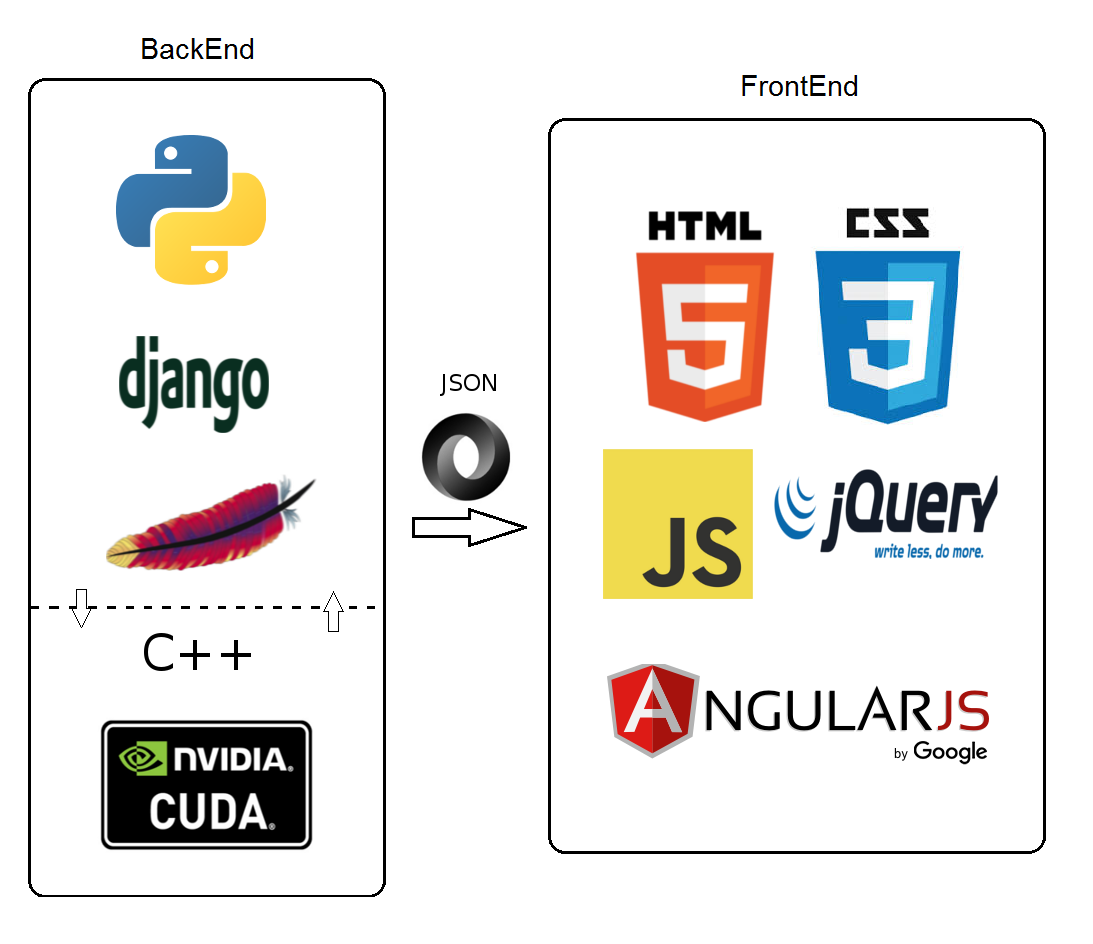
\includegraphics[width=1\linewidth]{../images/estructura}
	\caption[Estructura del sistema]{Estructura del sistema}
	\label{fig:estructura}
\end{figure}



\newpage
\section{Partes del sistema}

\bigskip
\textbf{BackEnd}\\

Será el lado del servidor de la aplicación. Basado en Django (y disponible mediante el servidor Apache), con éste tenemos acceso a los recursos del servidor, entre ellos la GPU. Con Django formaremos la petición según los parámetros que ha especificado el cliente, y se hará uso de la GPU mediante CUDA. Django tendrá la salida del cálculo, y la devolverá en un formato determinado.

Se puede decir que el BackEnd tiene 2 partes: el servidor web y el procesado dentro del servidor.

\bigskip
\textbf{FrontEnd}\\

Lado que ve el cliente, el FrontEnd. Con las tecnologías básicas web (HTML5, CSS y JavaScript) se creará una interfaz para el cliente. Mediante jQuery y AngularJS podrá interactuar fácilmente y con fluidez, además de servir la respuesta que le da el servidor.

\bigskip
AngularJS se encarga de la comunicación con el BackEnd a través de servicios, y con esos datos actualiza la interfaz. Conforma un modelo MVC (Modelo Vista Controlador), que separa los datos y su gestión (componente de modelo) de la aplicación de la interfaz de usuario (vista) y el módulo encargado de gestionar los eventos y las comunicaciones (controlador).

MVC propone la construcción de tres componentes distintos (modelo, vista y controlador): por un lado define componentes para la representación de la información, y por otro lado para la interacción del usuario. 

\bigskip
\begin{figure}[h]
	\centering
	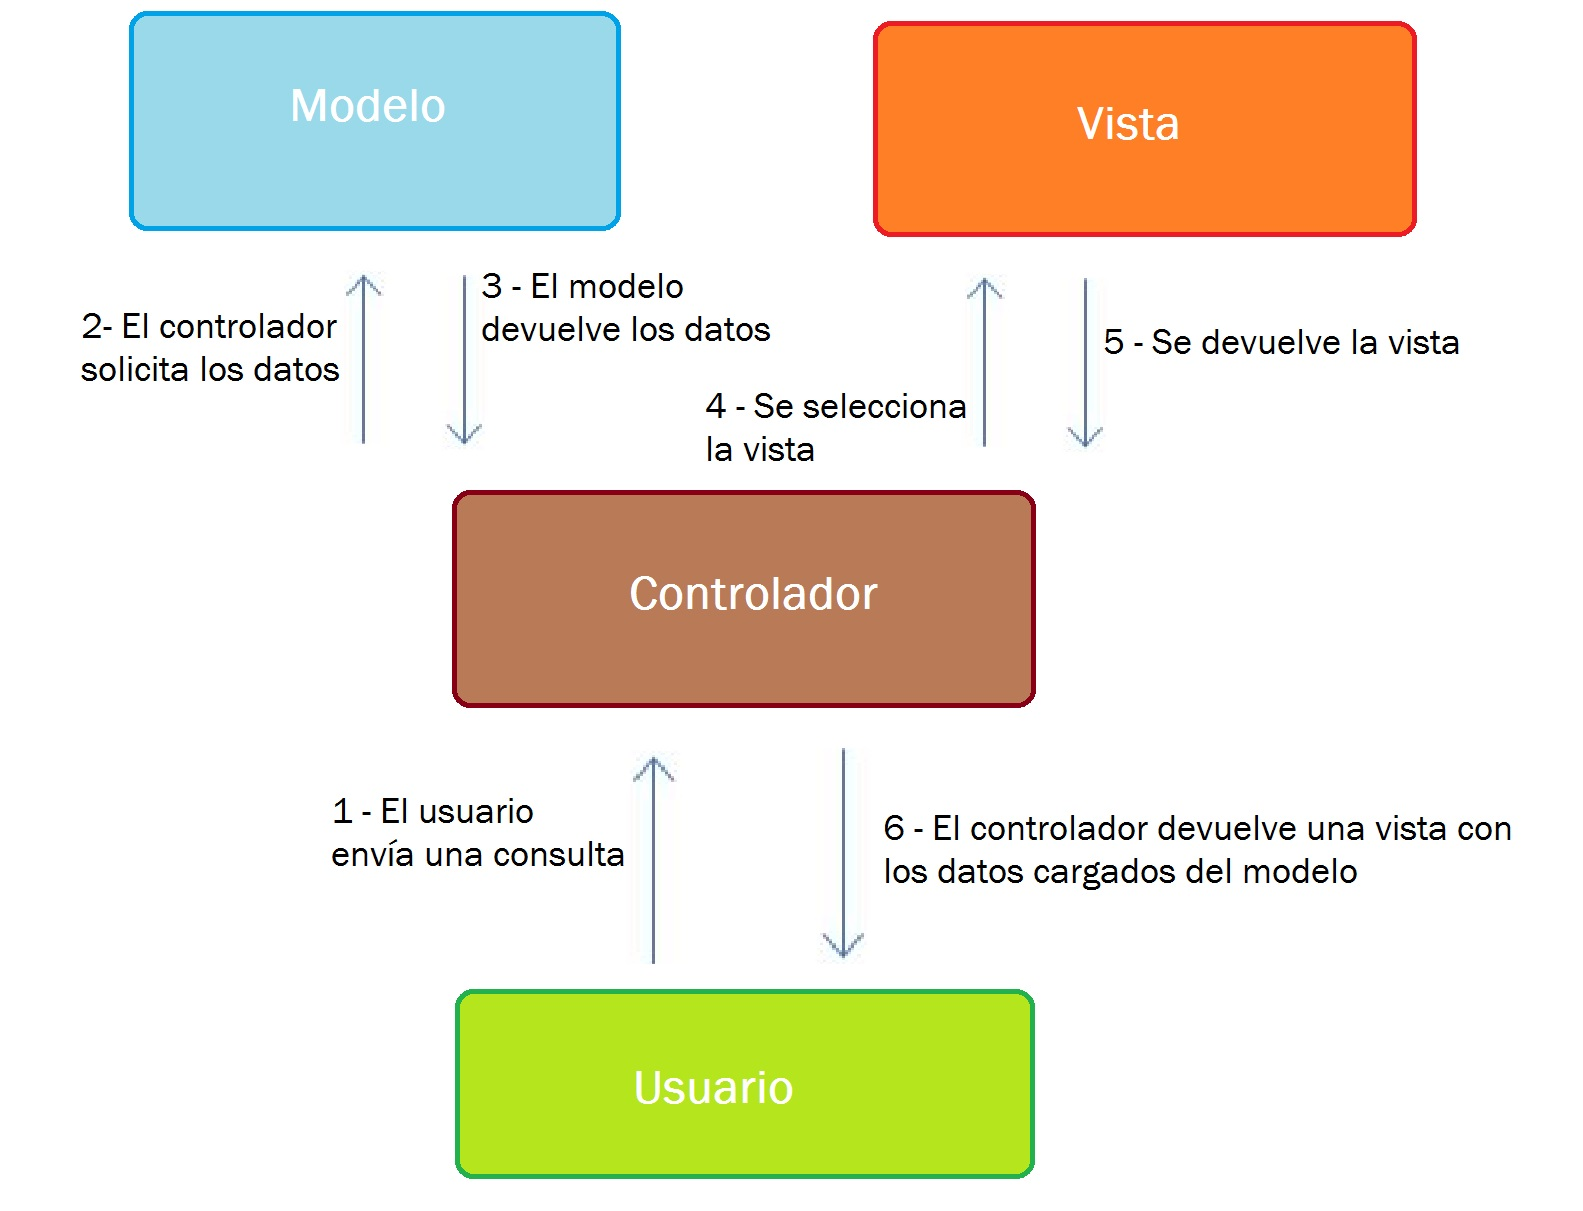
\includegraphics[width=0.8\linewidth]{../images/mvc}
	\caption[Modelo Vista Controlador]{Modelo Vista Controlador}
	\label{fig:mvc}
\end{figure}



\newpage
\section{Filosofía a seguir}
\bigskip
A la hora de implementar y de realizar el trabajo en general se ha intentado ser lo más ordenado y pulcro posible, esto en un principio  puede ralentizar el proceso, pero a largo plazo hace que el desarrollo, actualización o mantenimiento del sistema sea más rápido y fácil. Estos son algunos de los criterios empleados en el desarrollo.

\bigskip
\subsection{Desarrollo general}
\bigskip

Las funciones del sistema se han desarrollado de la manera más general posible para así favorecer la reutilización de código y facilitar su legibilidad. También son más fáciles de mantener puesto que al ser de ámbito más general son más mantenibles.

\bigskip
\subsection{Modularización}
\bigskip

Se ha desarrollado el código en distintos módulos. De esta forma se evita que al hacer cambios en un módulo se propague a los demás, lo que hace el código más mantenible y eficiente.

\bigskip
\subsection{Control de versiones}
\bigskip

Se apostó por un sistema de control de versiones, en mi caso Git mediante la plataforma GitHub \cite{github}, ya que favorece el mantenimiento de las distintas versiones de código de una manera sencilla y rápida.

El manejo de Git es sencillo, ya que con unas cuantas ordenes se puede manejar sin problemas, y GitHub está provisto de una interfaz muy intuitiva. 

\bigskip
Algunas de las órdenes que se han usado para el trabajo son:\\


\textit{git clone[URL del proyecto]}: se descarga el proyecto del repositorio Git.\\


\textit{git add [archivos]}: añade los archivos con los cambios deseados en un "paquete" para el commit.\\


\textit{git commit}: subida de los archivos especificados al repositorio local.\\


\textit{git push}: propaga los cambios locales al repositorio.\\


\textit{git pull origin}: Actualiza la versión del código.\\


\textit{git status}: muestra el estado de los archivos.\\


\bigskip
\subsection{Desarrollo iterativo incremental}
\bigskip

El desarrollo de las funcionalidades se hace de forma progresiva, de modo que primero se implementan las más críticas y prioritarias en primer lugar para poder tener siempre un producto funcional.

\bigskip
\subsection{Revisiones periódicas del código}
\bigskip

El código es revisado tras cada interacción de desarrollo, con el fin de mantenerlo lo más pulcro y estructurado posible. De este modo se evitan repeticiones en el código o dejar partes incompletas. Así se proporciona un mayor nivel de calidad a código producido.

\bigskip
\subsection{Documentación del código}
\bigskip

El código ha sido documentado, de modo que es más mantenible por terceros y por el mismo autor. Cada funcionalidad ha sido detallada debidamente, de manera clara y concisa, sin extender demasiado la explicación.




\newpage
\section{Estructura}

\bigskip
\subsection{FrontEnd}
\bigskip

Sigue el modelo que recomienda AngularJS, como antes se cita, se basa en el modelo MVC. Los distintos tipos de archivos que formarán las \textit{vistas} (en distintas ubicaciones según la forma de Django) son:

\begin{itemize}
	\item HTML (dentro del directorio \textit{templates}) será la plantilla visible del sistema.
	\item CSS: (en el directorio \textit{static/assets/css}) estilos que usará HTML.
	\item JavaScript (dentro de \textit{static/assets/js}) mediante jQuery y AngularJS permitirán interactuar con el sistema.
	\item Las imágenes y distintas librerías que se usen también se ubicarán en \textit{static/assets}.
\end{itemize}


\bigskip
\subsection{BackEnd}
\bigskip

Se hará uso de Django para crearlo y gestionarlo. A continuación se citan sus partes importantes que se usan en el proyecto:

\begin{itemize}

	\item \textbf{manage.py}: archivo para gestionar el proyecto (inspeccionarlo en busca de problemas, lanzar el servidor o cargar datos).
	\item \textbf{settings.py}: configuraciones del proyecto (dirección de algunos directorios o carga de módulos con distintas funcionalidades)
	
	Dentro del directorio \textit{swgpu} (que será un \textit{packete python}):
	\begin{itemize}
		\item \textbf{urls.py}: URL declaradas dentro del proyecto \textit{swgpu}.
		\item \textbf{views.py}: para gestionar las vistas y las funcionalidades del proyecto.
	\end{itemize}
	
	
	\item La parte de FrotEnd antes descrita se situará en los directorios \textit{templates} y \textit{static}. Django hará uso de los distintos archivos dentro para lanzar y trabajar con el servicio web.
\end{itemize}

\bigskip
\subsection{Ejecutable a usar por el BackEnd}
\bigskip

El sistema hará uso de la GPU del servidor (BackEnd) mediante el ejecutable \textit{geneticAlgorithm} (ubicado en el directorio \textit{bin}), escrito en C++ y CUDA. De esta manera se facilitará el servicio, ya que al tratarse de un ejecutable al que sólo hay que realizar una petición con los parámetros deseados se cubren los posibles fallos y la salida que dará. 

\bigskip
En las siguiente imagen se ve una captura de petición de ayuda sobre las variables a introducir mediante el ejecutable:

\bigskip
\begin{figure}[h]
	\centering
	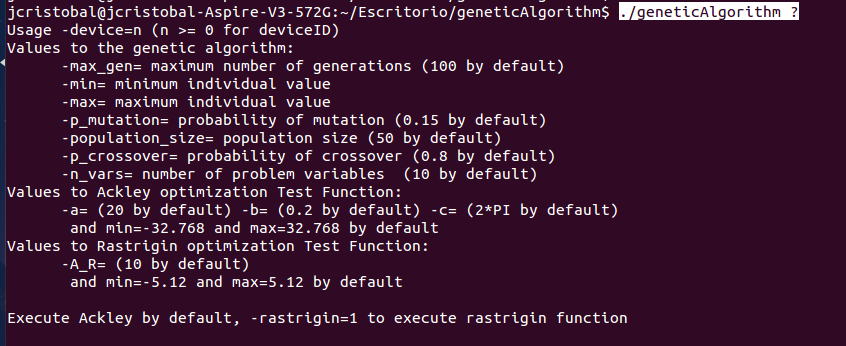
\includegraphics[width=1\linewidth]{../images/peticion_ejecutable}
	\caption[Petición de un algoritmo genético mediante el ejecutable]{Petición de un algoritmo genético mediante el ejecutable}
	\label{fig:peticion_ejecutable}
\end{figure}

\bigskip
Y otra captura con una petición que ejecutaría el algoritmo genético con los parámetros especificados además de los declarados por defecto:

\bigskip
\begin{figure}[h]
	\centering
	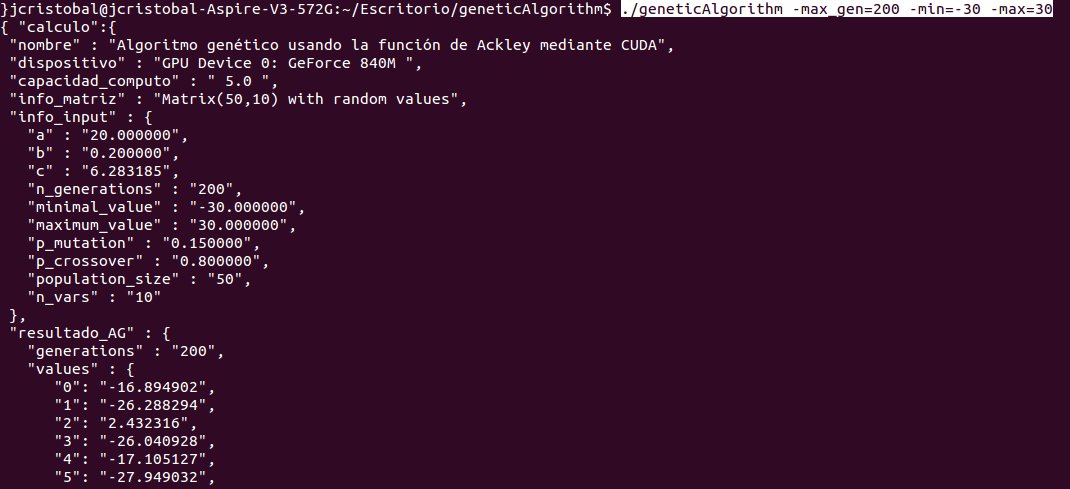
\includegraphics[width=1\linewidth]{../images/salida_ejecutable}
	\caption[Salida del algoritmo genético]{Salida del algoritmo genético}
	\label{fig:salida_ejecutable}
\end{figure}

\bigskip
y a continuación se ve la salida completa en formato JSON:

\begin{lstlisting}
{
	"calculo": {
		"nombre": "Algoritmo genético usando la función de Ackley mediante CUDA",
		"dispositivo": "GPU Device 0: GeForce 840M ",
		"capacidad_computo": " 5.0 ",
		"info_input": {
			"a": "20.000000",
			"b": "0.200000",
			"c": "6.283185",
			"n_generations": "200",
			"minimal_value": "-30.0000",
			"maximum_value": "30.0000",
			"p_mutation": "0.150000",
			"p_crossover": "0.800000",
			"population_size": "50",
			"n_vars": "10"
		},
		"resultado_AG": {
			"generations": "200",
			"values": {
				"0": "-16.894902",
				"1": "-26.288294",
				"2": "2.432316",
				"3": "-26.040928",
				"4": "-17.105127",
				"5": "-27.949032",
				"6": "25.647144",
				"7": "-7.420090",
				"8": "-0.034110",
				"9": "13.586363"
			},
			"best_fitness": "0.000000"
		},
		"datos_computo": {
			"performance": "9846.59 Flop/s",
			"time": "50.779 msec",
			"size": "500 ps",
			"workgroupSize": "50 threads/block"
		}
	}
}
\end{lstlisting}


\bigskip
Se optó por un ejecutable porque si cada vez que se realizara una petición hubiese que compilar el programa con el algoritmo genético, comprobar que no hubiese fallos ni generase errores, y no se garantizaría una salida formateada correctamente, además de generar una petición que consume más recursos y tiempo.

\bigskip
Pese a todas esas desventajas, se podría permitir al usuario cambiar el código fuente, o añadir funcionalidades y con un buen uso por su parte y una correcta prevención de fallos se conseguiría una funcionalidad mayor y llena de posibilidades. Pero como esta posibilidad no se ofrece en este trabajo, se hablará en el capítulo 8 sobre ella.


\newpage
\section{Pruebas}
\bigskip

A continuación se probará el rendimiento en 2 dispositivos distintos con sus respectivas especificaciones para realizar el cómputo. Con esto se verá que el sistema no depende de un modelo específico de tarjeta y presenta buenos resultados para varios modelos.

Se probará para una tarjeta GeForce 840M \cite{geforce840m} y GeForce GXT 660 Ti \cite{geforcegtx660}. Primero se verá una comparativa entre ambas, para luego ver los resultados obtenidos al realizar los mismo cómputos.

\bigskip
\begin{figure}[h]
	\centering
	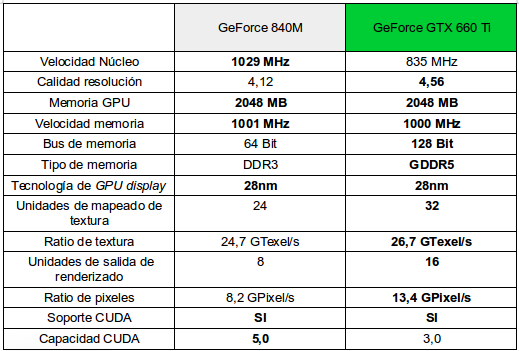
\includegraphics[width=1\linewidth]{../images/especificaciones}
	\caption[Especificaciones de las tarjetas 840M y GTX660]{Especificaciones de las tarjetas 840M y GTX660}
	\label{fig:especificaciones}
\end{figure}

\bigskip
Como nota hay que destacar el parámetro de \textit{capability} (capacidad), que será el que mayores restricciones o mejoras imponga en sus distintas versiones. Cuanto mayor sea esta, más funcionalidades podrá realizar y soportará más requisitos técnicos.

\bigskip
En la siguiente gráfica (Figura \ref{fig:grafico_benchmarks}) se verá la diferencia de ambas en benchmarks para medir \underline{procesamiento de gráficos} (Parallax, MRender, Gravity y Splatting):

\begin{figure}[h]
	\centering
	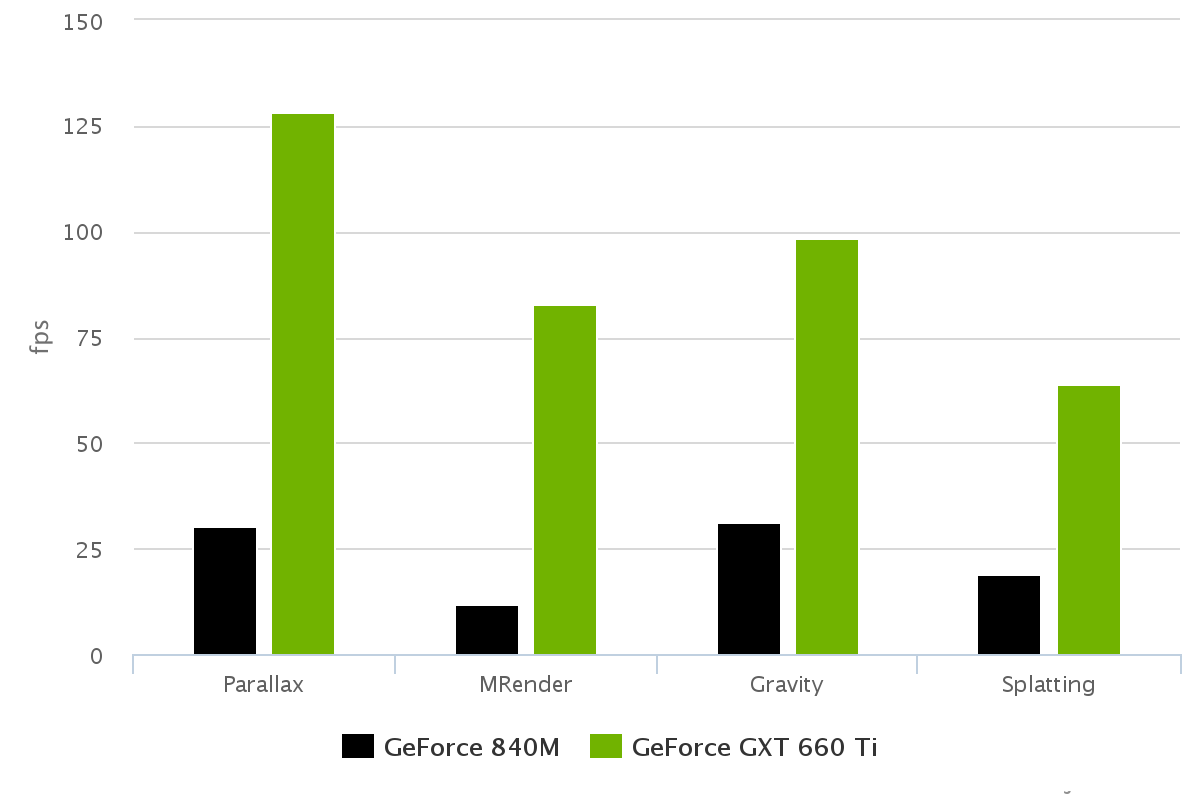
\includegraphics[width=0.6\linewidth]{../images/grafico_benchmarks}
	\caption[Comparativa de las tarjetas mediante bencharks de GPU]{Comparativa de las tarjetas mediante bencharks de GPU}
	\label{fig:grafico_benchmarks}
\end{figure}


\newpage %\bigskip
Pero en el ámbito de la computación mediante GPU con CUDA tendremos hay que fijarse en la capacidad de cada modelo de tarjeta, ya que una versión más actualizada puede lograr mejores resultados aunque tenga peores especificaciones \cite{capacidadescuda}.

\bigskip
Para ello se verán los tiempos que emplean ambas tarjetas (con distintas capacidades \cite{capacidades}) para varios números de generaciones:

\bigskip
\begin{figure}[h]
	\centering
	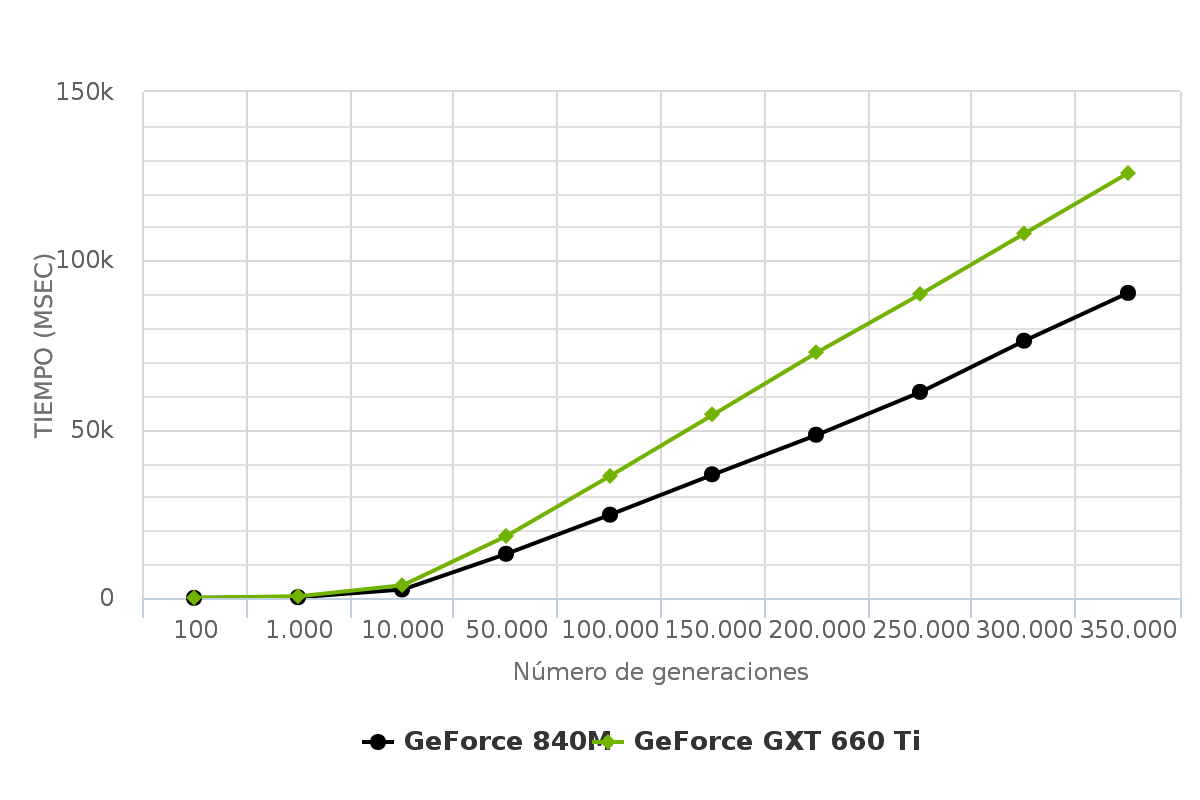
\includegraphics[width=0.9\linewidth]{../images/grafico_tiempos}
	\caption[Comparativa de tiempos entre tarjetas]{Comparativa de tiempos entre tarjetas}
	\label{fig:grafico_tiempos}
\end{figure}

\bigskip
Y se ve que la tarjeta con mejores prestaciones pero peor capacidad (GeForce GTX 660 Ti) tarda más en ejecutar los mismos procesamientos que hace la tarjeta con peores prestaciones pero mejor capacidad (GeForce 840M).

\bigskip
Como conclusión se llega a que a la hora de escoger el dispositivo a usar por el sistema para realizar los cómputos no sólo habrá que tener en cuenta los requisitos, si no que el factor de capacidad será decisivo para el rendimiento del cómputo y con ello del sistema.

También que ambas producen buenos resultados en el sistema, por lo que, se podría usar cualquiera en el sistema.


\chapter{Manuales}


\section{Manual de usuario}
\bigskip

El cliente o usuario tendrá una primera impresión de la \textit{portada} del servicio web. Simplemente se le mostrará el logo y título del servicio y podrá avanzar hacia las funcionalidades mediante un botón, o haciendo \textit{scroll} hacia abajo.

\bigskip
\begin{figure}[h]
	\centering
	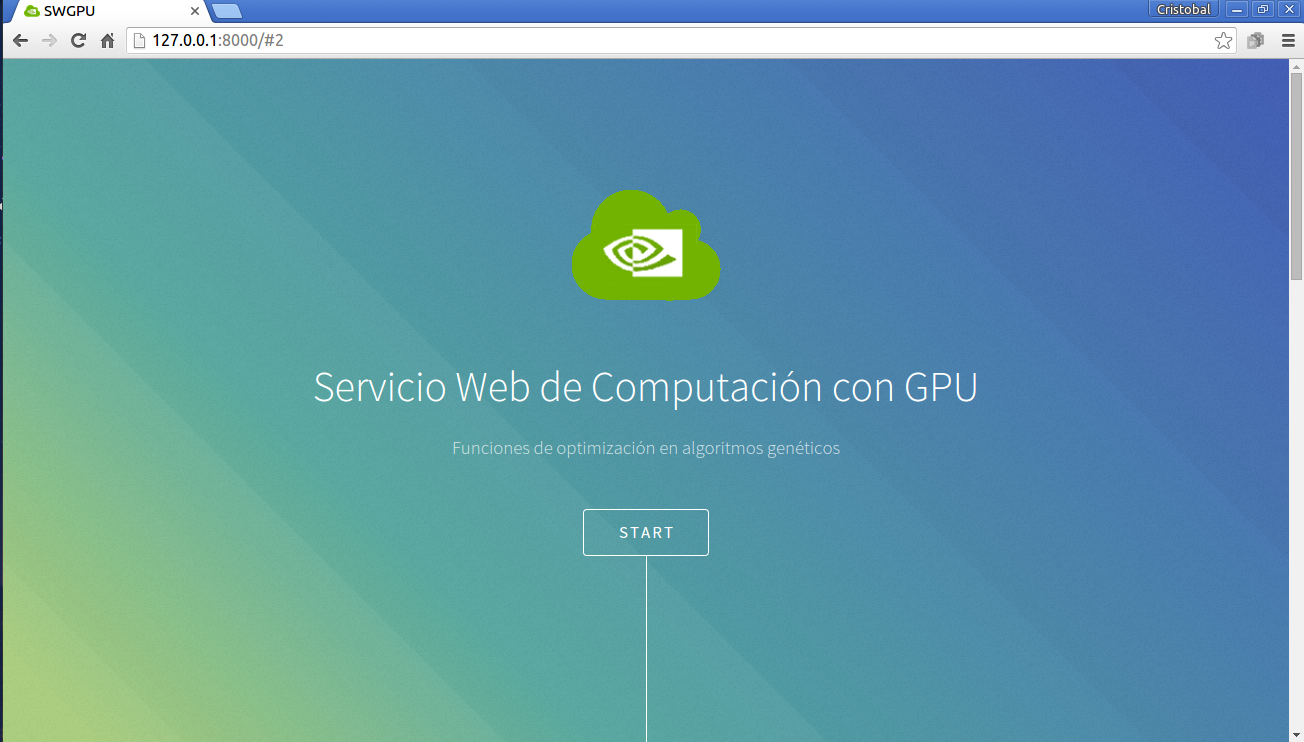
\includegraphics[width=1\linewidth]{../images/captura_web_1}
	\caption[Captura de la portada del servicio web]{Captura de la portada del servicio web}
	\label{fig:captura_web_1}
\end{figure}


Una vez avance podrá ver los servicios disponibles: ejecutar un algoritmo genético y que use la funcion de evaluacion de Ackley o de Rastrigin. Para acceder a dichos servicios sólo tendrá que \textit{clickar} sobre el servicio que quiera y se desplegará.

\bigskip
\begin{figure}[h]
	\centering
	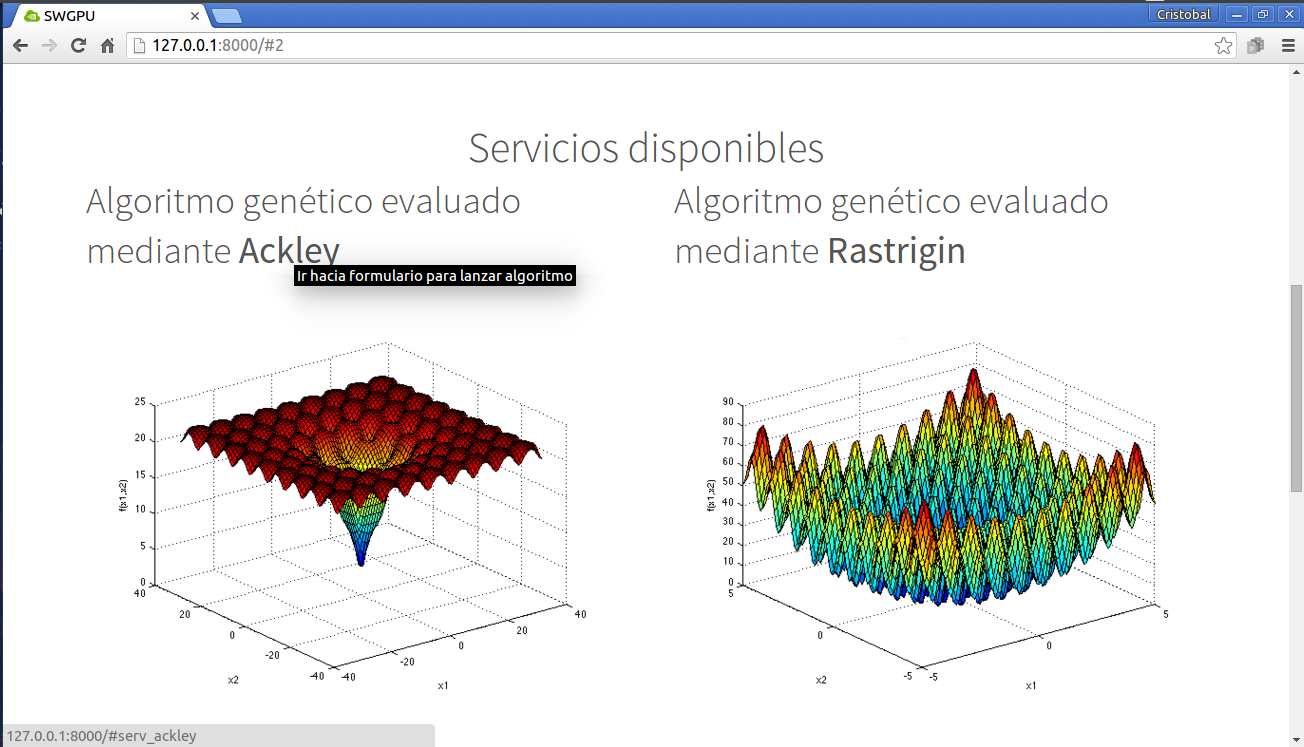
\includegraphics[width=0.9\linewidth]{../images/captura_web_2}
	\caption[Captura de los servicios disponibles]{Captura de los servicios disponibles}
	\label{fig:captura_web_2}
\end{figure}


\bigskip
Una vez elegido el servicio se desplegará su correspondiente formulario. Para acceder a él el usuario sólo tendrá que \textit{clickar} sobre el título en la pantalla de \textit{Servicios disponibles} o avanzar hacia el mediante \textit{scroll}. Una vez en el formulario se le mostrarán los valores por defecto de cada parámetro, pudiendo cambiar cada uno de manera sencilla:

\bigskip
\begin{figure}[h]
	\centering
	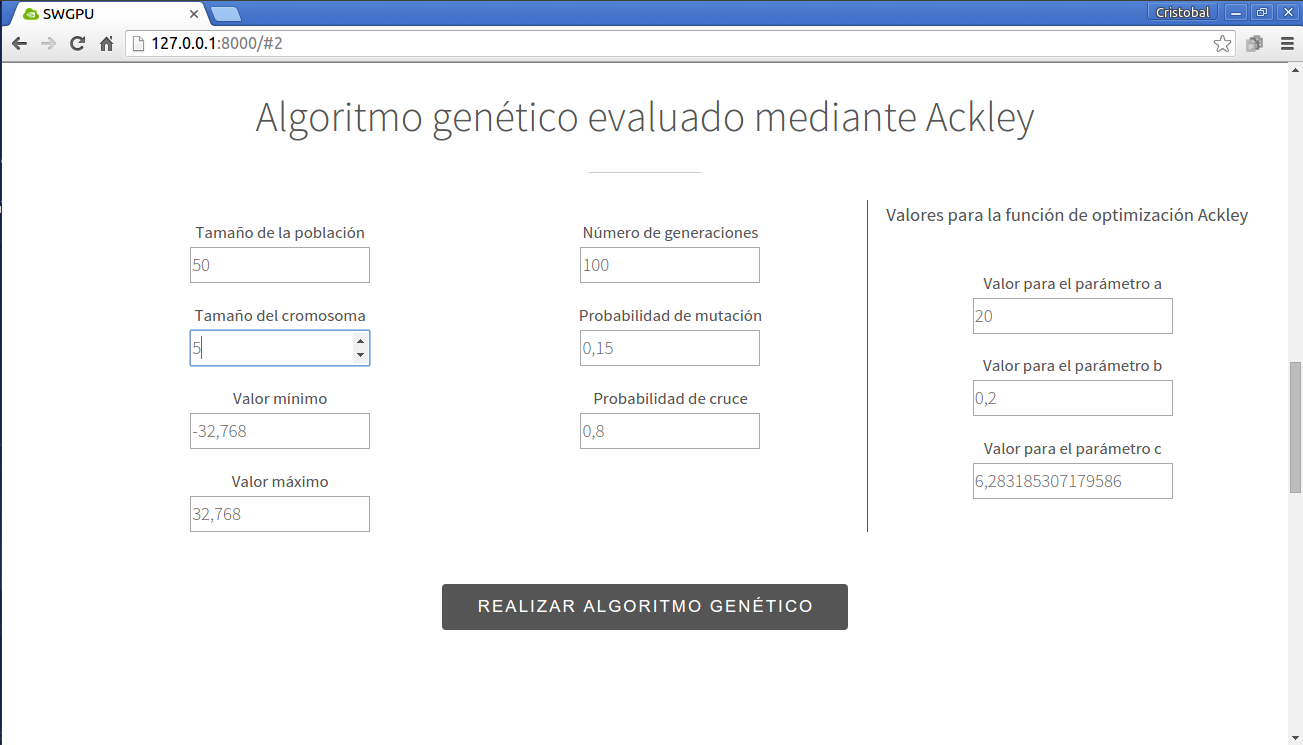
\includegraphics[width=0.9\linewidth]{../images/captura_web_3}
	\caption[Formulario para lanzar el algoritmo genético]{Formulario para lanzar el algoritmo genético}
	\label{fig:captura_web_3}
\end{figure}

\bigskip
También se asegurará que se introducen los valores correctamente:

\bigskip
\begin{figure}[h]
	\centering
	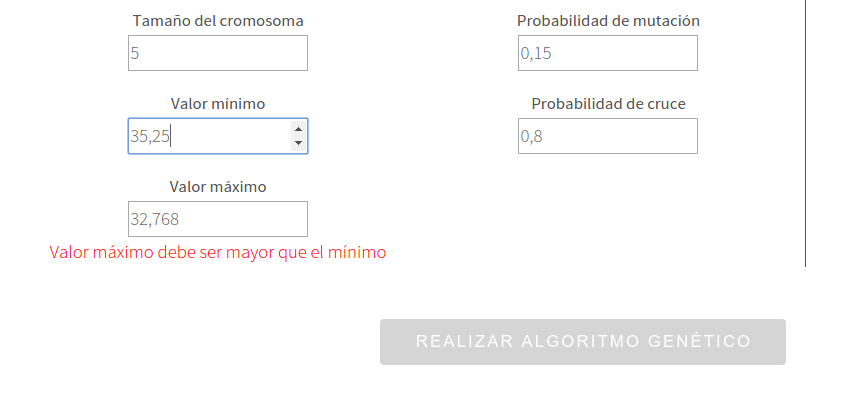
\includegraphics[width=0.7\linewidth]{../images/captura_web_3_1}
	\caption[Mensaje de error en el formulario]{Mensaje de error en el formulario}
	\label{fig:captura_web_3_1}
\end{figure}


\bigskip
Y una vez realizado el algoritmo genético, ya se podrá acceder a los resultados. Para ello sólo hay que avanzar hacia abajo o mediante el botón de V\textit{er resultados}. Se mostrará información sobre la petición (hora y parámetros), datos sobre el cómputo (dispositivo usado o tiempo invertido) y los resultados obtenidos.

\bigskip
\begin{figure}[h]
	\centering
	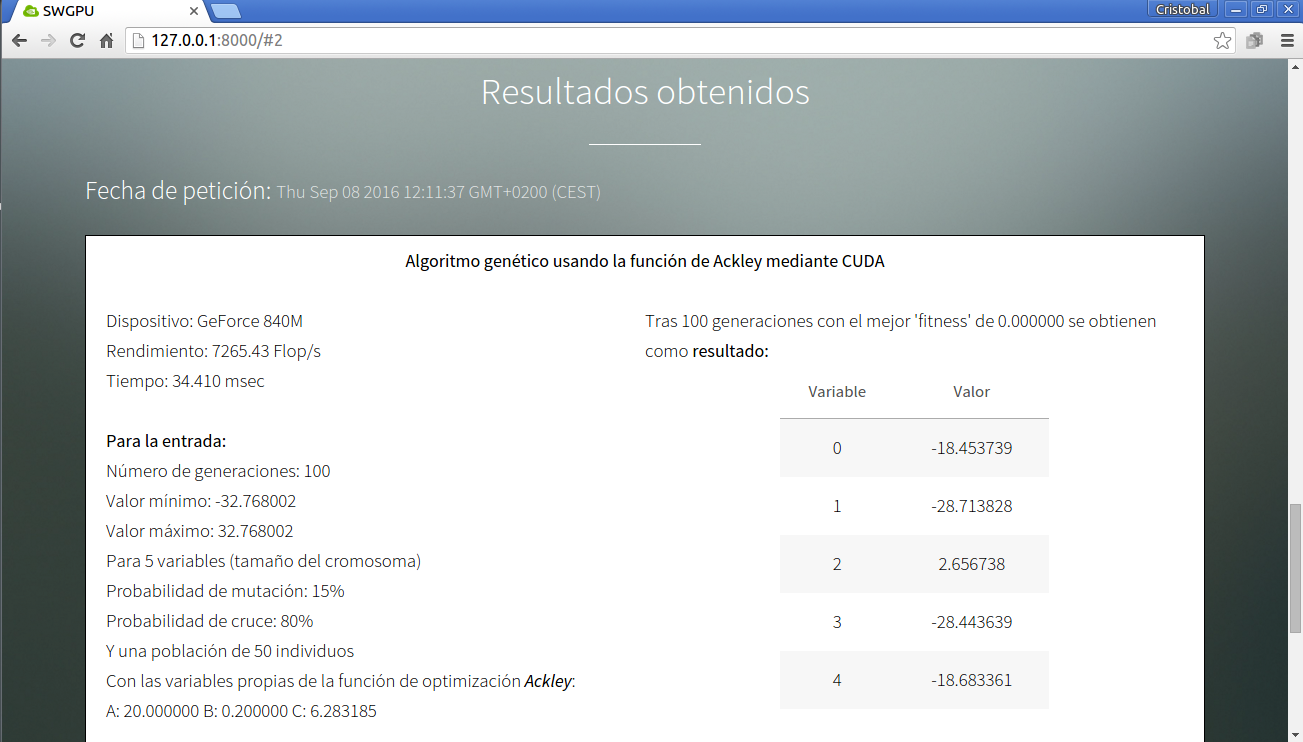
\includegraphics[width=1\linewidth]{../images/captura_web_4}
	\caption[Resultados obtenidos]{Resultados obtenidos}
	\label{fig:captura_web_4}
\end{figure}


\newpage
\bigskip
Por último se muestra al final (aunque se puede acceder siempre a él) una sección de contacto. Se podrá poner en contacto con el administrador del sistema.

\bigskip
\begin{figure}[h]
	\centering
	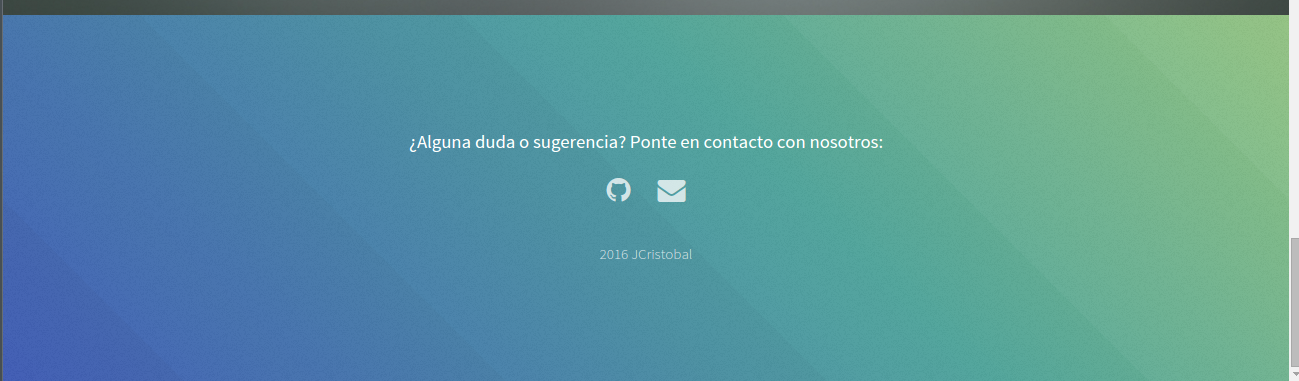
\includegraphics[width=0.9\linewidth]{../images/captura_web_5}
	\caption[Sección de contacto]{Sección de contacto}
	\label{fig:captura_web_5}
\end{figure}


\bigskip
Además, como añadido, se facilita la ayuda sobre parámetros y ejecución del ejecutable \textit{geneticAlgorithm} como parte independiente, sin requerir del servicio web, como se puede ver en la Figura \ref{fig:peticion_ejecutable} del capitulo anterior.


\newpage
\section{Manual de despliegue}
\bigskip

A continuación se explicará la forma y requisitos de despliegue del sistema. 

\subsection{Requisitos para el despliegue}
\bigskip

Para el correcto despliegue de la aplicación habrá que contar con sus 2 partes: el servicio web y el procesamiento con GPU mediante CUDA.

\bigskip
Para lanzar el servicio web:
\begin{itemize}
	\item Apache (versión 2.4 o superior)
	\item Python (Python 2)
	\item Django  (versión 1.10 o superior)
\end{itemize} 

\bigskip
Y para el procesamiento mediante CUDA:
\begin{itemize}
	\item Dispositivo NVIDIA
	\item Drivers NVIDIA (versión 352.xx)
	\item CUDA 7.5
	\item C++ (versión 4.x)
\end{itemize} 

\subsection{Despliegue}
\bigskip


Una vez que se cumplen los requisitos, sólo habrá que lanzar el servicio web, ya que el procesamiento usando la GPU se gestiona mediante el ejecutable \textit{geneticAlgorithm} dirigido por el servicio web.

Para ello el servidor Apache tendrá que estar activo (se puede activar ejecutando \textit{service apache2 restart}) y lanzar el proyecto Django con el proyecto: dentro del directorio SWGPU ejecutar, junto con la URL donde lanzar el sistema \textit{python manage.py runserver [URL]}


\subsection{Despliegue automatizado}
\bigskip
También se proporcionará el script o archivo \textit{despliegue.sh} para automatizar la tarea de despliegue.

Simplemente habrá que ejecutarlo (dentro del \textit{directorio SWGPU},mediante la orden \textbf{sudo ./despliegue.sh}) y luego especificar la URL donde se desplegará. El script comprobará los requisitos antes citados, preparará el servidor y lanzará el sistema.

En la siguiente captura se ve como se lanza el servidor:

\bigskip
\begin{figure}[h]
	\centering
	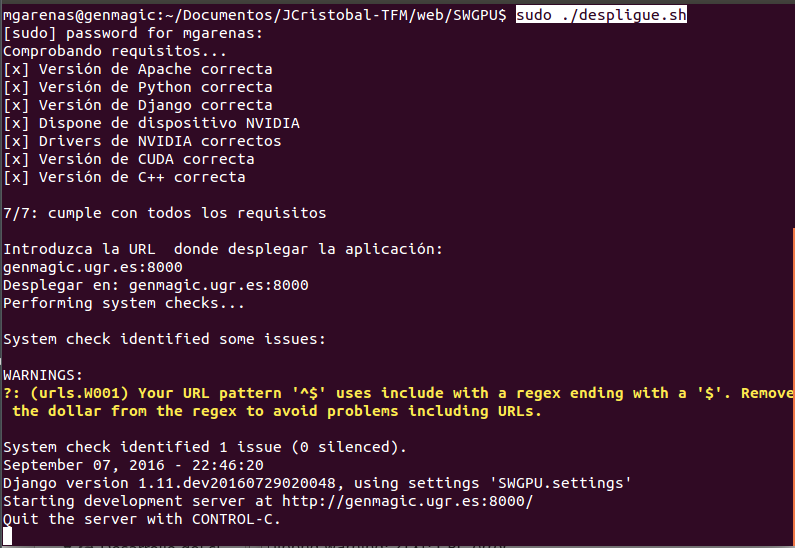
\includegraphics[width=1\linewidth]{../images/prueba_despliegue}
	\caption[Captura del despliegue automático]{Captura del despliegue automático}
	\label{fig:prueba_despliegue}
\end{figure}



\chapter{Conclusiones y trabajos futuros}


\bigskip
\section{Conclusiones}
\bigskip

Una vez realizado el trabajo, se verán los objetivos (citados en el capítulo 2) y su respectivo avance.

\bigskip
Respecto a las clases para lanzar un algoritmo genético se han logrado cumplir, reuniéndolas en el archivo ejecutable \textit{geneticAlgorithm}. Se ha desarrollado como un módulo independiente, para poder ser usado por cualquier servicio, y no ser dependiente del servicio web, controlando la entrada de parámetros y control de fallos.

\bigskip
También se ha creado la estructura del servicio web, de manera que sea accesible desde cualquier servidor web.
Dicho servicio facilita la petición del algoritmo genético, y se obtendrán los resultados mediante el uso de la GPU del servidor.

\bigskip
Se a publicado el servicio, en forma de \textit{beta}. Se encuentra accesible en  \href{www.genmagic.ugr.es:8000}{www.genmagic.ugr.es:8000}, accesible dentro de la red de la UGR \cite{vpnugr}.
	

\section{Trabajos futuros}

\bigskip
Además de mantener y gestionar la versión actual del servicio web, se podría trabajar en la mejora de la experiencia de usuario.

\bigskip
También se refinará el algoritmo, logrando un mejor aprovechamiento de los recursos y mejorando los resultados.

\bigskip
Como se comenta en el capítulo 6 (en la subsección \textit{Ejecutable a usar por el BackEnd}) se estudiará la posibilidad de que el usuario pudiera añadir funcionalidades o cualquier procesamiento usando la GPU mediante CUDA. 

\bigskip
De esta manera se podría ejecutar cualquier opción de optimización, o fuera del ámbito de los algoritmos genéticos cualquier funcionalidad que requiera el usuario.

\bigskip
Esto requeriría un conocimiento mayor por parte del usuario. Además supondría un mayor consumo de recursos, pero con un buen uso del usuario y una correcta prevención de fallos se conseguiría una funcionalidad mayor y llena de posibilidades. 











\newpage
%\bibliography{BIBLIO}
%\bibliographystyle{apalike}

%\bibliography{bibliografia}\addcontentsline{toc}{chapter}{Bibliografía}
%\bibliographystyle{ieeetr}

\bibliography{bibliografia}
\bibliographystyle{splncs}



\end{document}
